\documentclass[10pt]{beamer}

\usepackage[utf8]{inputenc}
\usepackage{graphicx}
\usepackage{amsmath}
\usepackage{newtxtext,newtxmath}
\usepackage{caption}
\usepackage{subcaption}
\usepackage{tabularx}
\usepackage{diagbox}
\usepackage{tikz}
\usepackage{pgf}

\providecommand{\main}{.}
\usepackage{\main/sty/slashbox}

\usetheme{Madrid}
% \usecolortheme{beaver}

% \setlength{\abovecaptionskip}{0pt}
\setlength{\belowcaptionskip}{0pt}

\graphicspath{{\main/img/}{\main/03_firmware/img/}{\main/ble_mesh/img/}{\main/04_hardware/img/}{\main/05_software/img/}{\main/06_result/img/}}

\title[INDOOR LOCALIZATION SYSTEM]{DESIGN AND IMPLEMENTATION OF INDOOR LOCALIZATION SYSTEM USING UWB AND WIRELESS MESH NETWORK}
\subtitle{Graduation Thesis}
\author[Ngo Van Tuan - 1613861]{Student: Ngo Van Tuan - 1613861\\
Supervisor: Dr. Vo Que Son
}
\institute[HCMUT]
{
  \inst{1}
%   VIETNAM NATIONAL UNIVERSITY HO CHI MINH CITY\\
%   HO CHI MINH CITY UNIVERSITY OF TECHNOLOGY\\
  FACULTY OF ELECTRICAL AND ELECTRONICS  ENGINEERING\\
  DEPARTMENT OF TELECOMMUNICATIONS ENGINEERING
}
\date{January 26, 2021}

% \logo{\pgfputat{\pgfxy(-1,7.5)}{\pgfbox[center,base]{
\includegraphics[width=1cm]{logoBK.png}}}}

\newcolumntype{g}{>{\columncolor{Gray}}c}
\newcolumntype{w}{>{\columncolor{white}}c}
\newcolumntype{L}{>{\arraybackslash}X}
\newcolumntype{M}[1]{>{\centering\arraybackslash}m{#1\textwidth}}

\newcommand{\myframetitle}[1]{\frametitle{\makebox[\framewidth]{#1 \hfill
\includegraphics[width=0.6cm]{logoBK.png}}}}

\begin{document}

\frame{\titlepage}

\begin{frame}
    \myframetitle{Table of Contents}
    \tableofcontents
\end{frame}

\AtBeginSection[]
{
  \begin{frame}
    \myframetitle{Table of Contents}
    \tableofcontents[currentsection]
  \end{frame}
}

% \begin{frame}
%     \frametitle{}
%     \begin{columns}
%         \column{0.5\textwidth}
%         \column{0.5\textwidth}
%     \end{columns}
% \end{frame}

\section{Introduction}

\begin{frame}
\myframetitle{Introduction: Outdoor vs Indoor Localization}
\begin{columns}
\column{0.5\textwidth}
Advantages of GPS:
\begin{itemize}
    \item Almost available anywhere
    \item Free to use
    \item Get calibrated by its own
    \item Provide location-based info
\end{itemize}
\begin{figure}[h]
    \begin{center}
        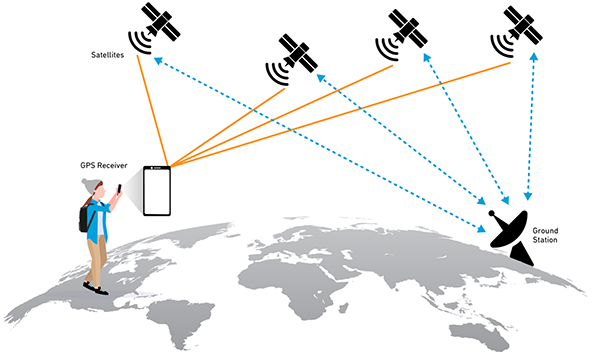
\includegraphics[width=1\textwidth]{gps.png}
    \end{center}
    \caption{Global Positioning System}
    \label{fig:gps}
\end{figure}
\column{0.5\textwidth}
Disadvantages of GPS:
\begin{itemize}
    \item Do not pierce through the solid walls or structures
    \item Not accurate enough for indoor applications
    % \item Not quick enough for realtime applications
\end{itemize}
\begin{figure}[h]
    \begin{center}
        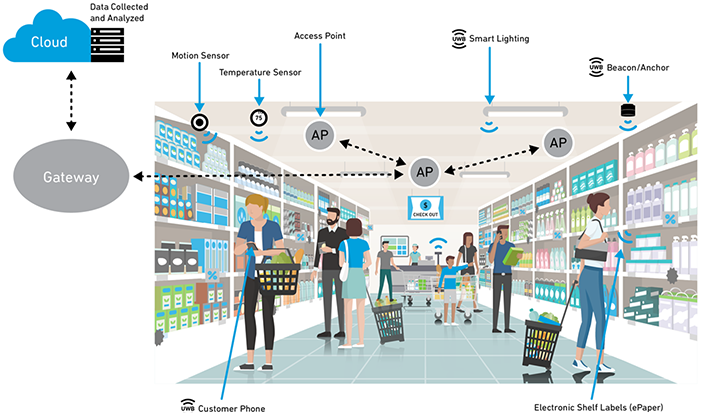
\includegraphics[width=1\textwidth]{ips.png}
    \end{center}
    \caption{Indoor Positioning System}
    \label{fig:ips}
\end{figure}
\end{columns}
\end{frame}

\begin{frame}
    \myframetitle{Introduction: Thesis Objective}
    % \frametitle{\makebox[\framewidth]{Introduction: Thesis Objective \hfill
\includegraphics[width=0.6cm]{logoBK.png}}}
    \begin{columns}
        \column{0.4\textwidth}
    \begin{itemize}
        \item Design and implement an indoor localization system using UWB
        \item Build a system to manage and control the localization system based on Bluetooth mesh network
        \item Provide IoT services for remote control and self-identification
    \end{itemize}
    \column{0.6\textwidth}
    \begin{figure}[H]
        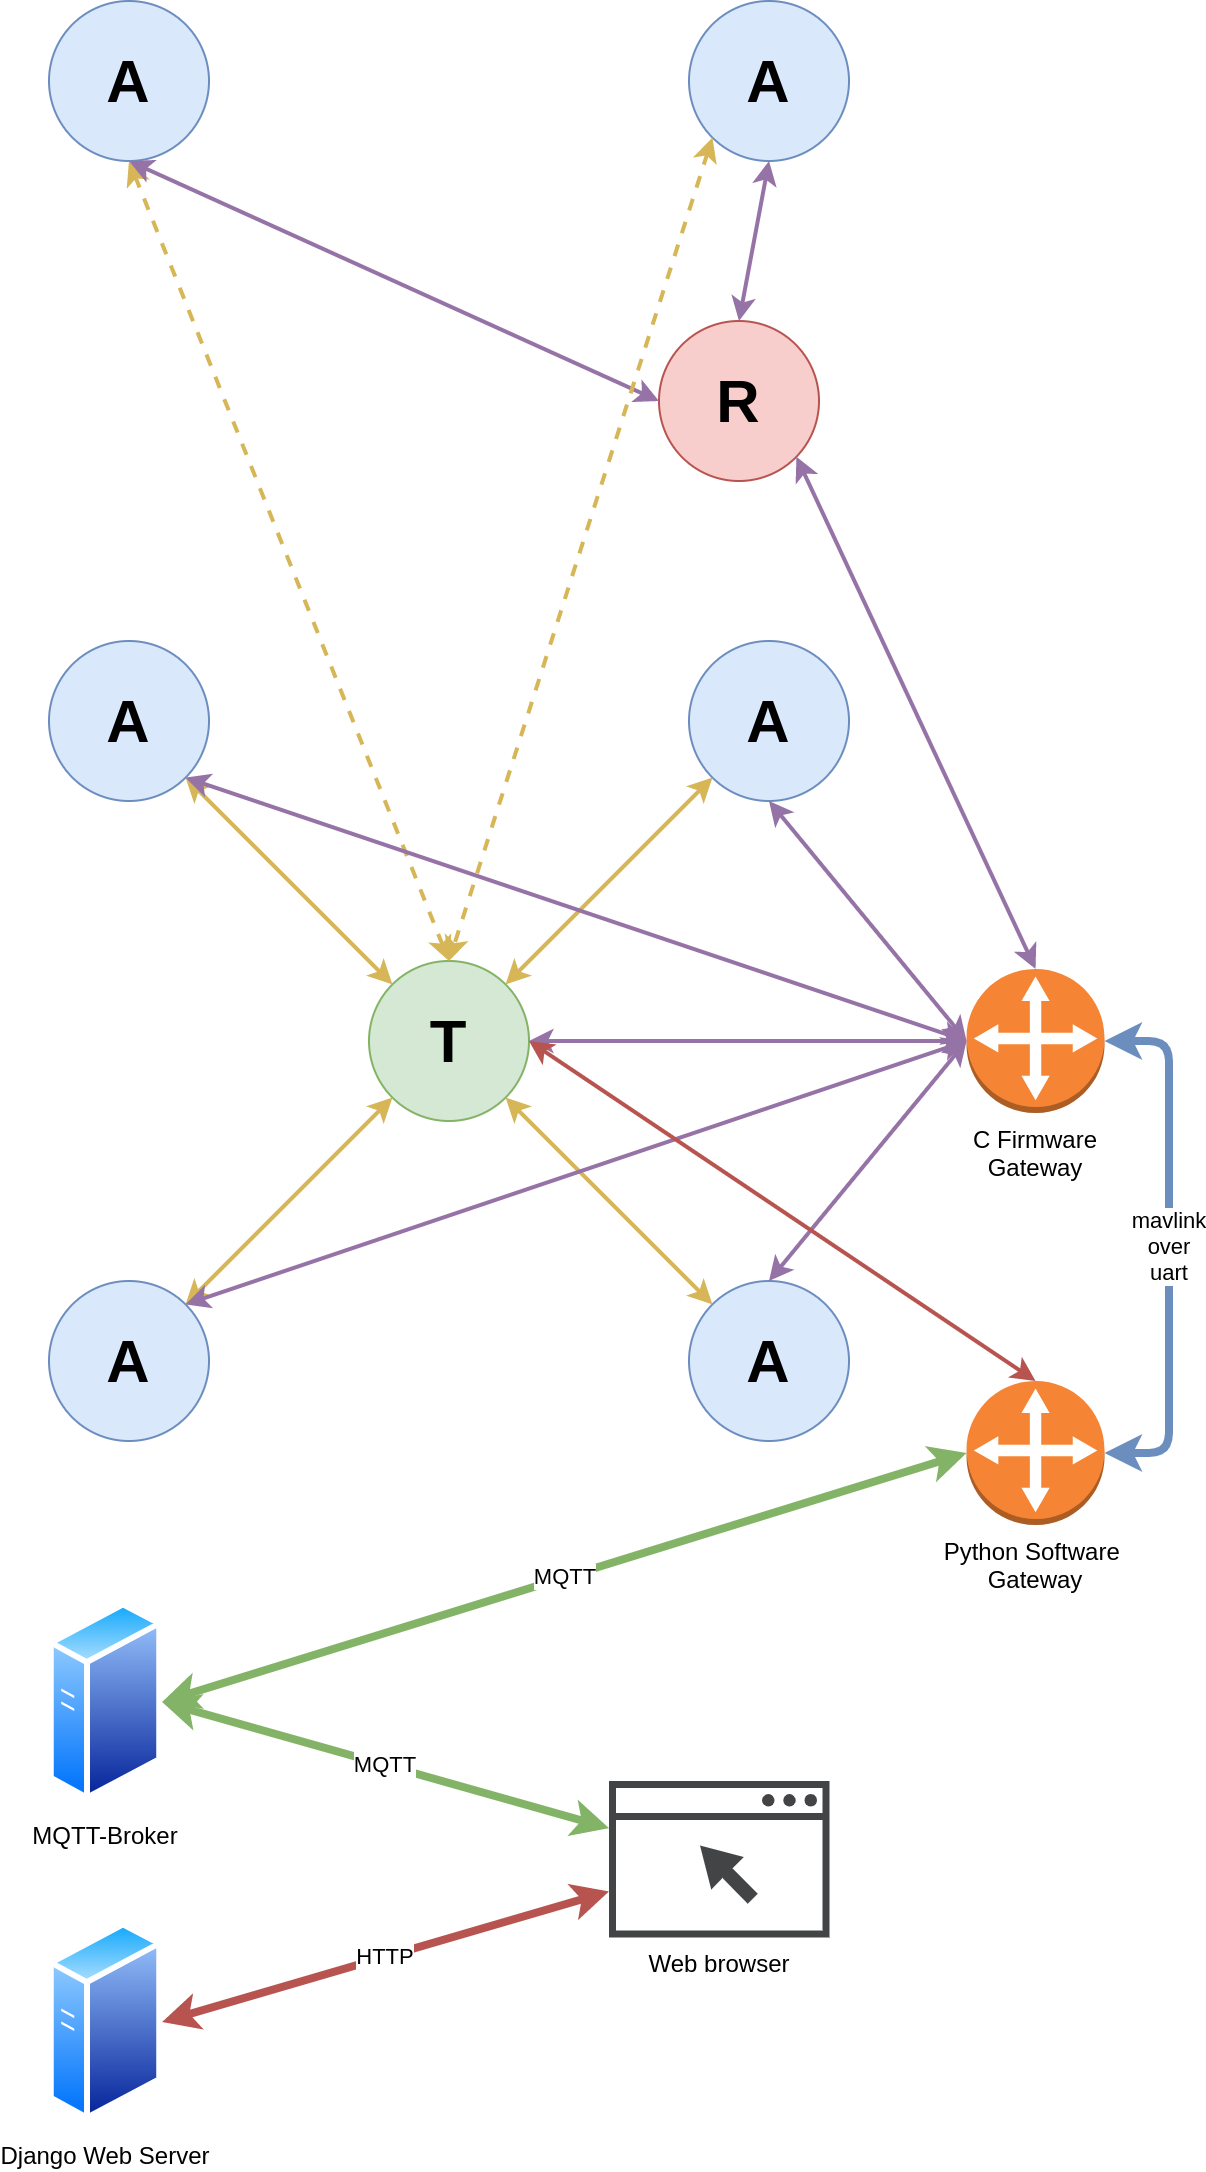
\includegraphics[width=0.8\textwidth]{system_overview.png}
        \caption{System overview}
        \label{fig:system_overview}
    \end{figure}
    \end{columns}
\end{frame}

\begin{frame}
    \myframetitle{Introduction: Ultra-Wideband}
    Definition of Ultra-Wideband signal:
\begin{columns}
    \column{0.3\textwidth}
    \begin{equation*}
        \begin{split}
            & B = (f\textsubscript{H} - f\textsubscript{L})\\
            & f\textsubscript{c} = \frac{f\textsubscript{H} + f\textsubscript{L}}{2}\\
            & B\textsubscript{frac} = \frac{B}{f\textsubscript{c}} = \frac{2(f\textsubscript{H} - f\textsubscript{L})}{f\textsubscript{H} + f\textsubscript{L}}
        \end{split}
    \end{equation*}
    \column{0.7\textwidth}
    \begin{figure}[H]
    \centering
    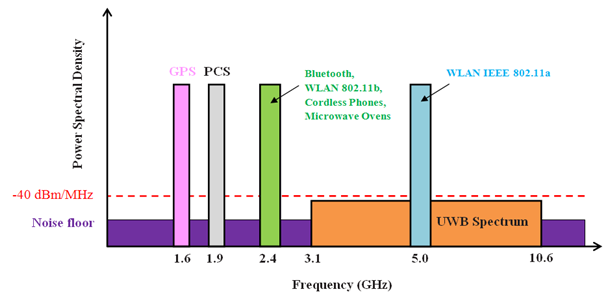
\includegraphics[width=1\textwidth]{uwb_versus_other_radio_communication_systems.png}
    \caption{UWB}
    \label{fig:uwb_versus_other_radio_communication_systems}
    \end{figure}
\end{columns}
Federal Communication Commission (FCC) has defined UWB signal:
\begin{itemize} 
    \item Absolute bandwidth greater than or equal 500Mhz, or
    \item $B$\textsubscript{frac} larger than 0.2
\end{itemize}
\end{frame}

\begin{frame}
    \myframetitle{Introduction: Why UWB + DWM1001?}
    Advantages of UWB:
    \begin{itemize}
        \item Potentially low complexity and low cost
        \item Noise like signal
        \item Resistant to multi-path and jamming
        \item Good time-domain resolution allowing for localization application
    \end{itemize}
    \begin{columns}
        \column{0.3\textwidth}
        \begin{figure}[H]
            \centering
            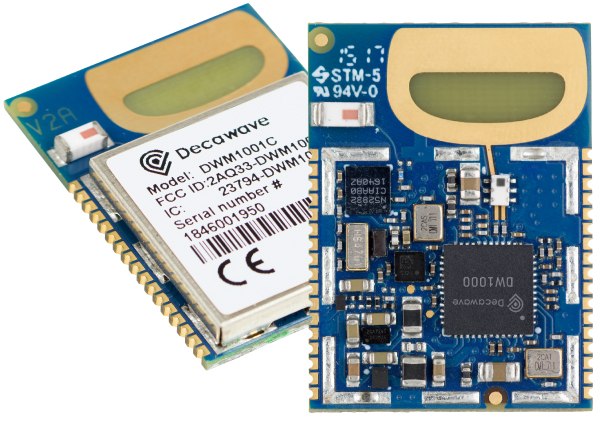
\includegraphics[width=1\textwidth]{DWM1001_Module_ProdPage_600x430.jpg}
            \caption{DWM1001 Module}
            \label{fig:DWM1001_Module_ProdPage_600x430}
        \end{figure}
        \column{0.7\textwidth}
        \begin{figure}[H]
            \centering
            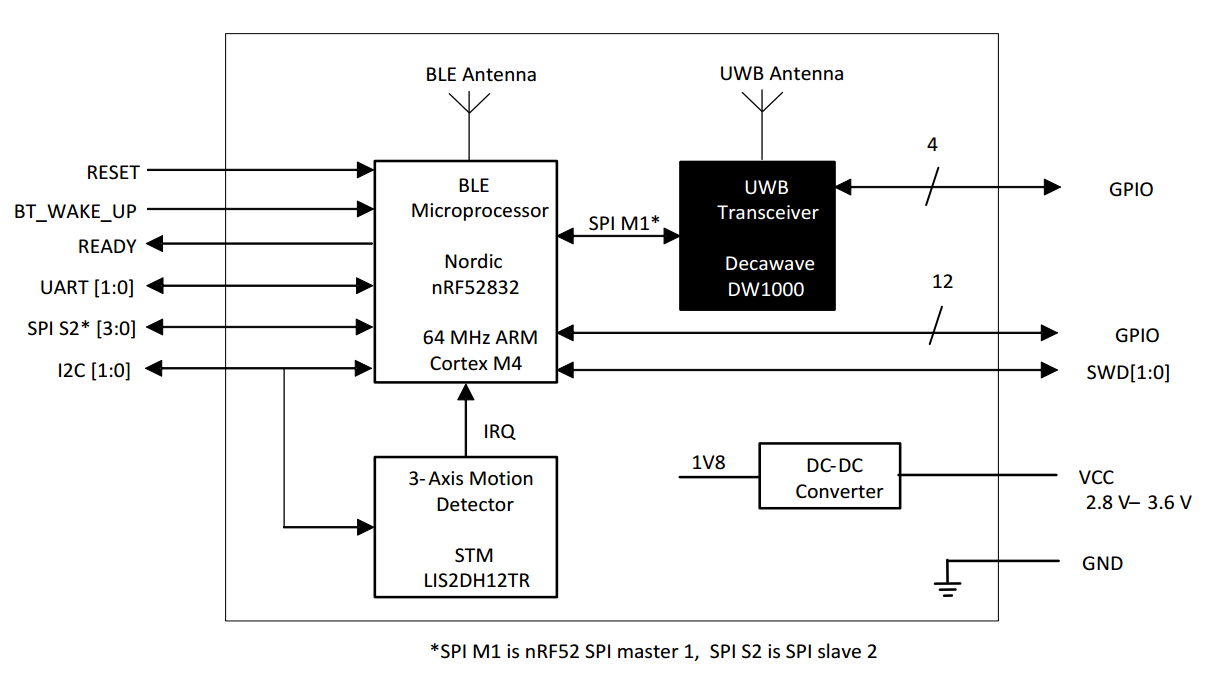
\includegraphics[width=1\textwidth]{dwm1001_block_diagram.png}
            \caption{DWM1001 block diagram}
            \label{fig:dwm1001_block_diagram}
        \end{figure}
    \end{columns}
\end{frame}

\section{Position estimation}

\begin{frame}
    \myframetitle{Position estimation: Two-Way Ranging}
    Time of Fight formula: 
    \begin{equation}
        tof = \frac{1}{2} ((tt2 - tt1) - (ta2 - ta1))
        \label{eqn:pos_est_twr_tof}
    \end{equation}
    \begin{columns}
        \column{0.3\textwidth}
        \begin{figure}[H]
            \centering
            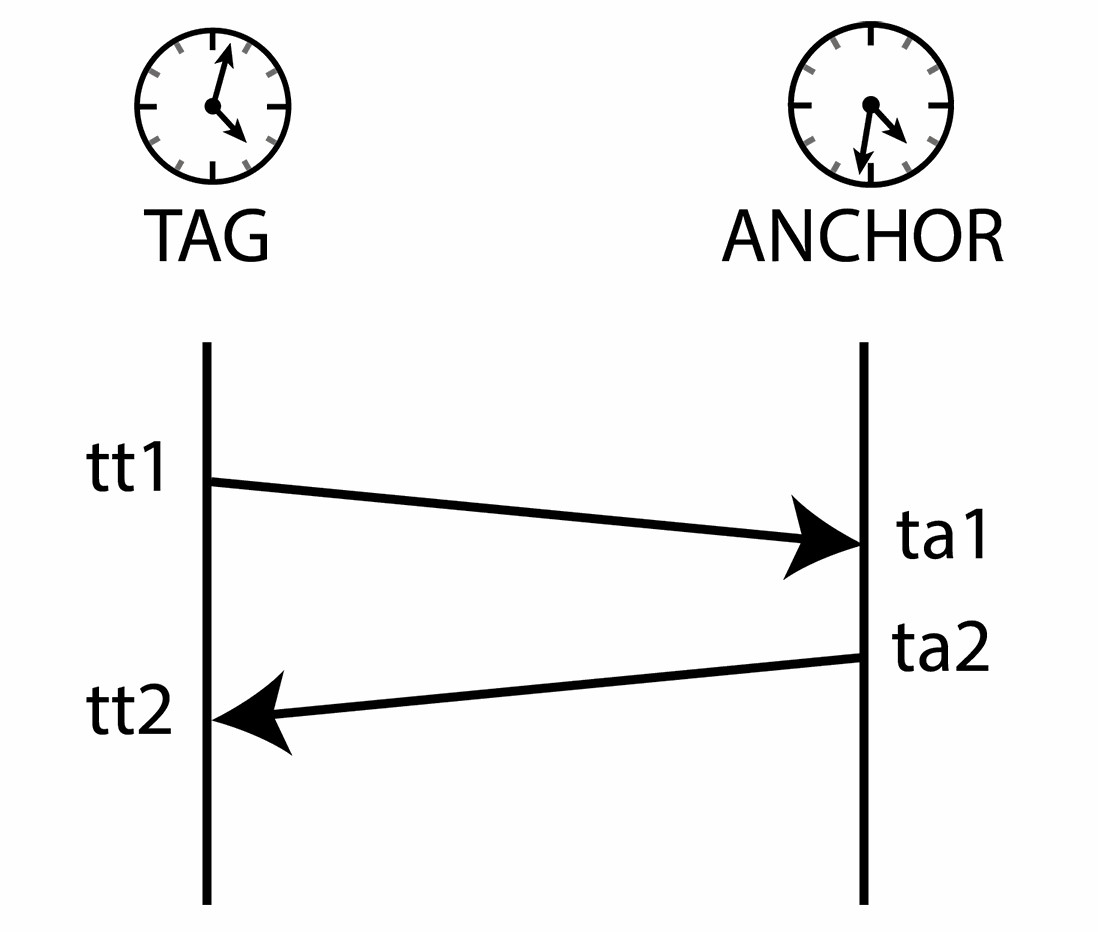
\includegraphics[width=1\textwidth]{twr_protocol.png}
            \caption{TWR}
            \label{fig:twr_anchor_and_tag}
        \end{figure}
        \column{0.7\textwidth}
        \begin{figure}[H]
            \centering
            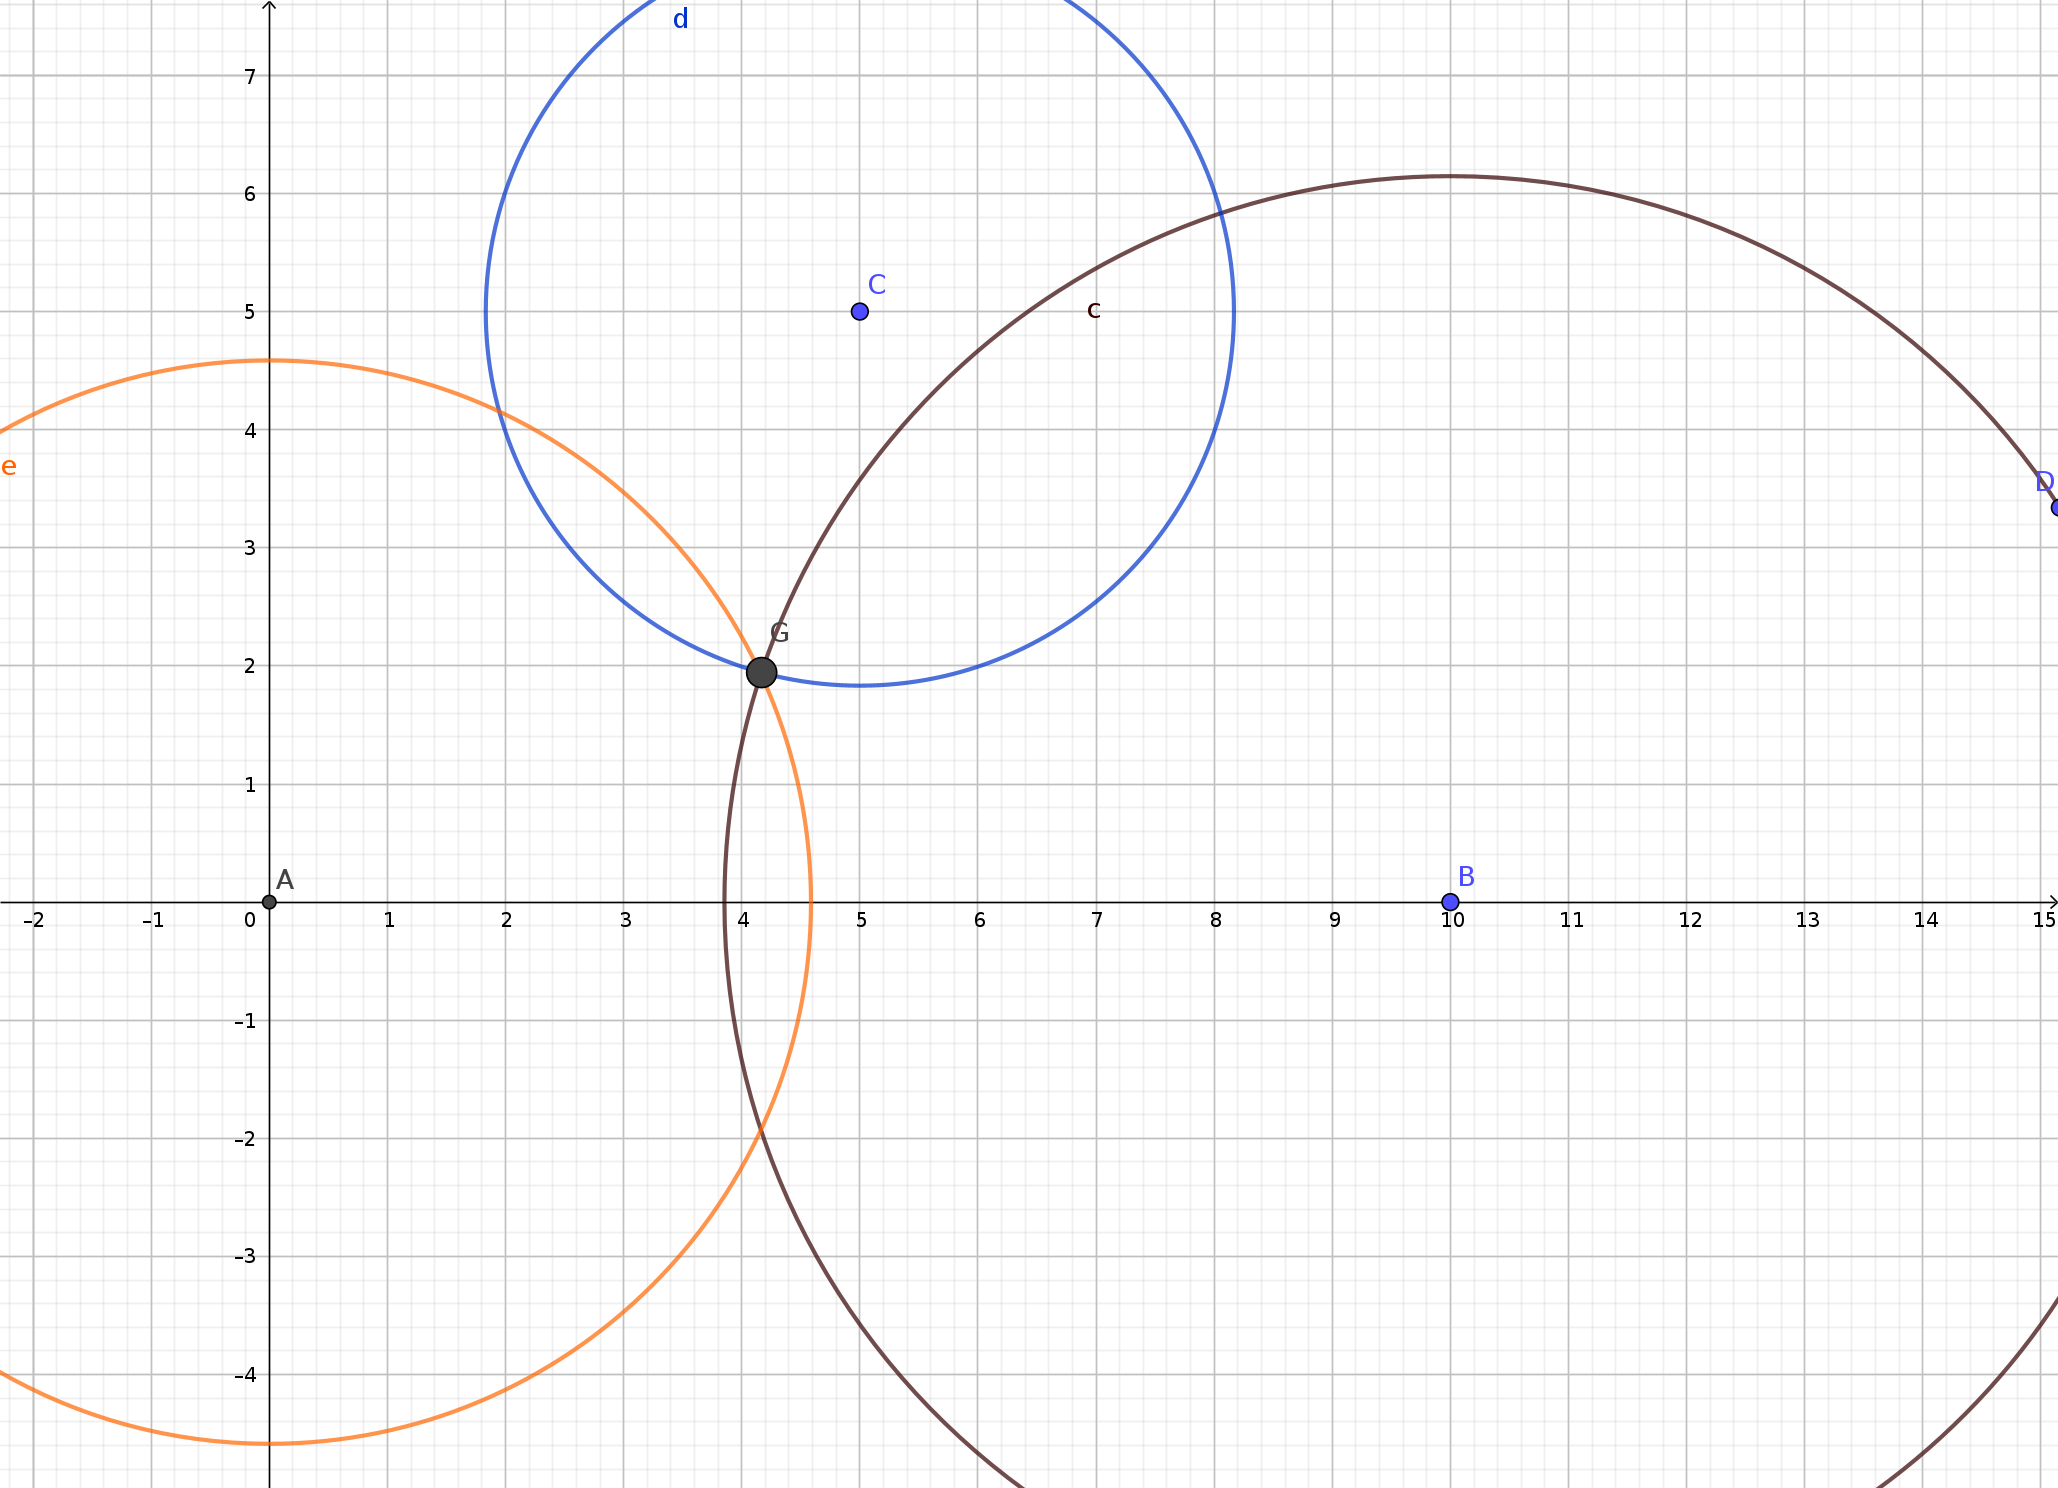
\includegraphics[width=0.8\textwidth]{twr.png}
            \caption{Localization using TWR}
            \label{fig:twr_trilateration}
        \end{figure}
    \end{columns}
\end{frame}

\begin{frame}
    \myframetitle{Position estimation: Multilateration}
    \begin{columns}
    \column{0.5\textwidth}
        \begin{columns}
            \column{0.2\textwidth}
            Anchors:
            \column{0.8\textwidth}
            $A_1(0,0,0)$\\
            $A_2(x_2,0,0)$\\
            $A_3(x_3,y_3,0)$
        \end{columns}
        \begin{columns}
            \column{0.2\textwidth}
            Tag:
            \column{0.8\textwidth}
            $T(x,y,z)$
        \end{columns}
        \begin{equation}
            \begin{split}
                d_1 = | T - A_1| \\
                d_2 = | T - A_2| \\
                d_3 = | T - A_3|
            \end{split}
        \end{equation}
        \begin{subequations}
            \begin{align}
                & x^2 + y^2 + z^2 = d_1^2 \label{eqn:d1_t_a_a}\\
                & (x-x_2)^2 + y^2 + z^2 = d_2^2 \label{eqn:d1_t_a_b}\\
                & (x-x_3)^2 + (y-y_3)^2 + z^2 = d_3^2 \label{eqn:d1_t_a_c}
            \end{align}
        \end{subequations}
    \column{0.5\textwidth}
        \begin{figure}[H]
            \centering
            \includegraphics[width=1\textwidth]{simplified_multilateration.png}
            \caption{Simplified multilateration}
            \label{fig:simplified_multilateration}
        \end{figure}
    \end{columns}
    \begin{columns}
        \column{0.4\textwidth}
        \begin{equation}
            \begin{split}
                x &= \frac{d_1^2 - d_2^2 + x_2^2}{2x_2}\\
                z &= \pm \sqrt{d_1^2 - x^2 - y^2} \\
            \end{split}
            \label{eqn:simplified_multilateration_x}
        \end{equation}
        \column{0.6\textwidth}
        \begin{equation}
            \begin{split}
                y &= \frac{d_1^2 - d_3^2 + x_3^2 + y_3^2 - \frac{x_3(d_1^2 - d_2^2 + x_2^2)}{x_2}}{2y_3}
            \end{split}
            \label{eqn:simplified_multilateration_z}
        \end{equation}
    \end{columns}
\end{frame}

\begin{frame}
    \myframetitle{Position estimation: Multilateration}
    \begin{columns}
        \column{0.4\textwidth}
        Closed-form Solution:
        \begin{equation}
            \begin{split}
            \boldsymbol{e_x} &= \frac{A_2-A_1}{\Vert A_2 - A_1\Vert} \\
            V_x &= \Vert A_3 - A_1 \Vert \cos{\gamma} \\
            &= \Vert \boldsymbol{e_x} \Vert \Vert A_3 - A_1 \Vert \cos{\gamma} \\
            &= \boldsymbol{e_x} \cdot (A_3 - A_1) \\
            \boldsymbol{e_y} &= \frac{A_3-A_1-(s*\boldsymbol{e_x})}{\Vert A_3-A_1-(s*\boldsymbol{e_x})\Vert} \\
            \boldsymbol{e_z} &= \boldsymbol{e_x} \times \boldsymbol{e_y}
            \end{split}
        \end{equation}

        \column{0.6\textwidth}
        \begin{figure}[H]
            \centering
            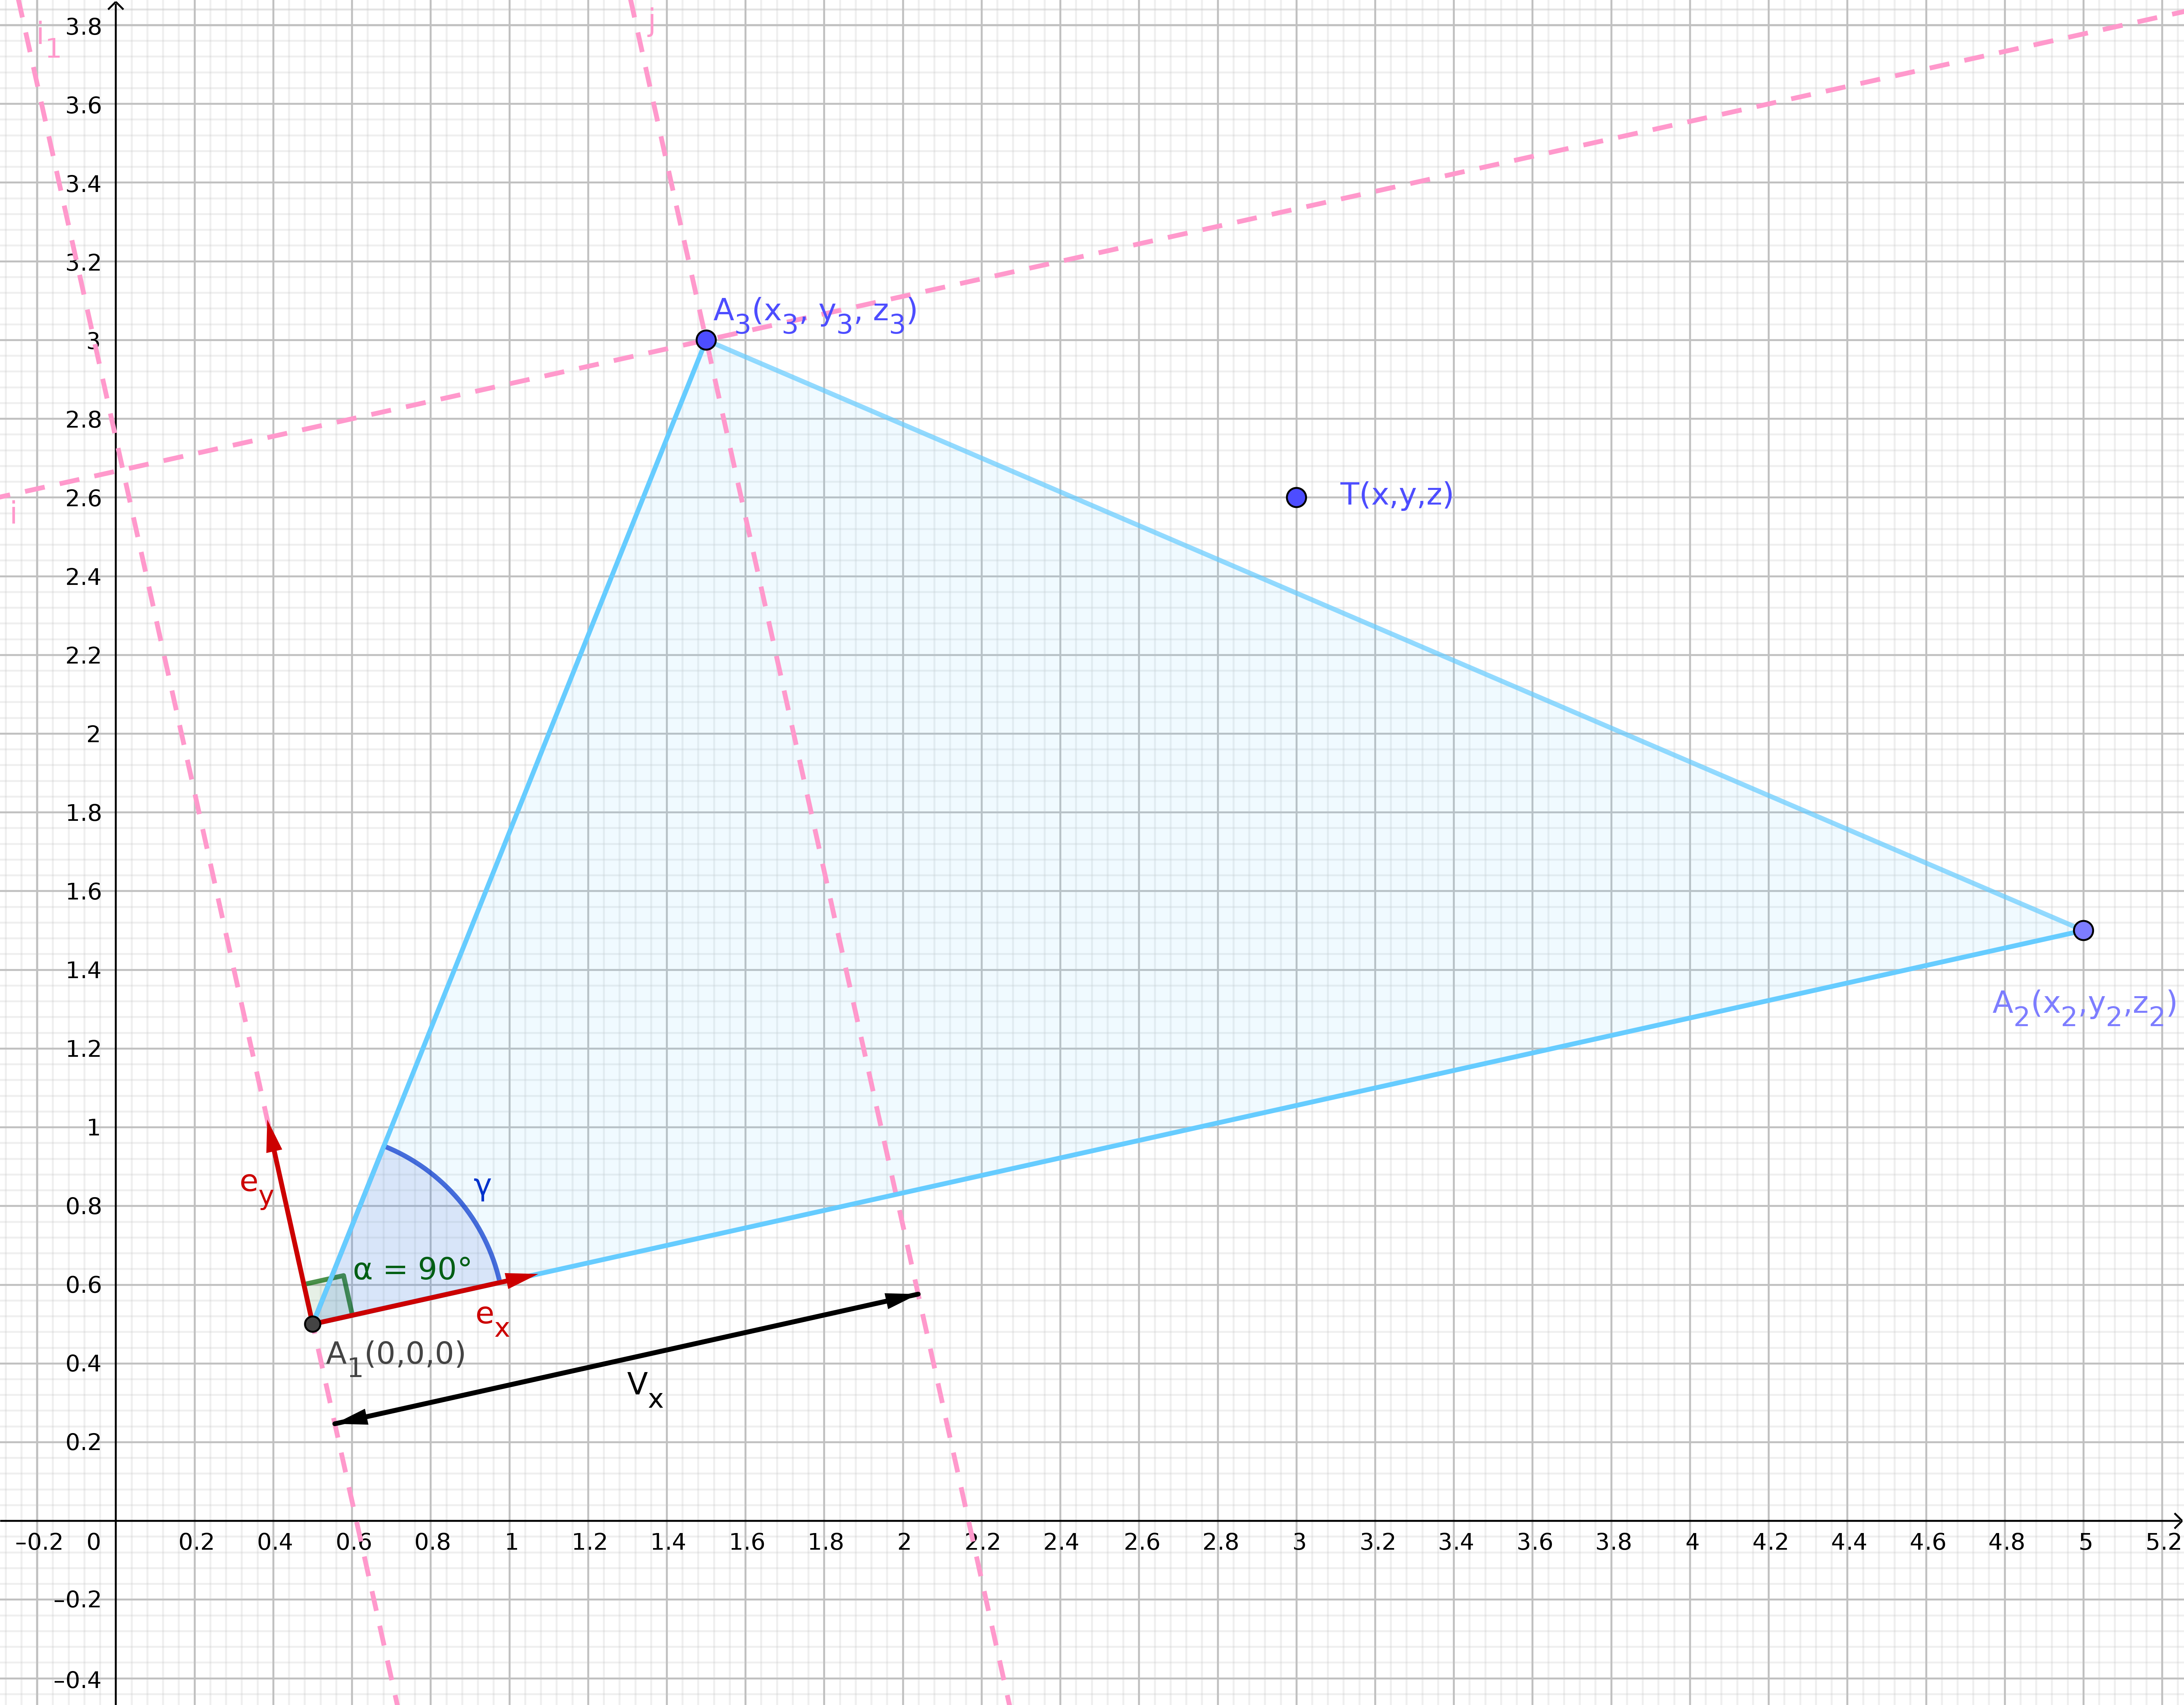
\includegraphics[width=0.8\textwidth]{multilateration.png}
            \caption{Multilateration in Euclidean space}
            \label{fig:multilateration}
        \end{figure}
    \end{columns}
    \begin{equation}
        \begin{split}
            &B_0(0,0,0) \\
            &B_1(U, 0, 0) = B_1(\Vert A_2 - A_1 \Vert, 0, 0) \\
            &B_2(V_x, V_y, 0) = B_2(\boldsymbol{e_x} \cdot (A_3 - A_1), \boldsymbol{e_y} \cdot (A_3 - A_1), 0) 
        \end{split}
        \label{eqn:multilateration_to_simplified_problem}
    \end{equation}
\end{frame}

\begin{frame}
    \myframetitle{Position estimation: ToF to Distance}
    \begin{figure}[H]
        \centering
        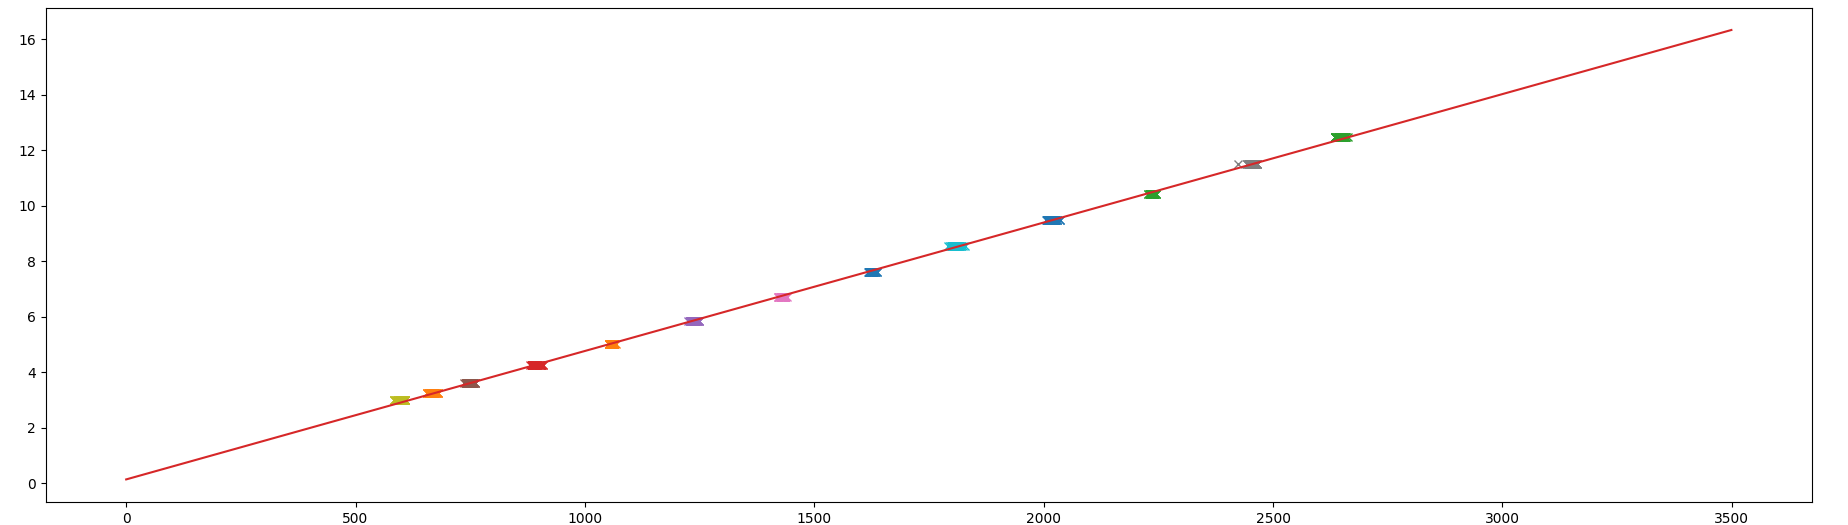
\includegraphics[width=1\textwidth]{tof_to_distance.png}
        \caption{ToF to distance}
    \end{figure}
    \begin{equation}
        d = w*ToF + b
        \label{eqn:distance_model}
    \end{equation}
    Using LinearRegression model of sklearn library:
    \begin{itemize}
        \item $w = 0.004632130984819555$: The slope of estimated model 
        \item $b = 0.13043560944811894$: The bias of estimated model
    \end{itemize}
    Mean error:
    \begin{equation*}
        e = \frac{1}{n} \sum_{k = 1}^{n} | d^k_{est}-d^k \vert = \frac{1}{n} \sum_{k = 1}^{n} | w*ToF^k + b -d^k \vert  = 0.04095793575440317 (m)
        \label{eqn:distance_model_loss}
    \end{equation*}
\end{frame}

\section{Ranging System Architecture}

\begin{frame}
    \myframetitle{RAS: Layered Architecture}
\begin{figure}[H]
    \begin{columns}
        \column{0.6\textwidth}
            3 layers model:
            \begin{itemize}
                \item CCP: Clock Calibration Packet
                \item TDMA: Time Division Multiple Access
                \item TWR: Two-Way Ranging
            \end{itemize}
        \column{0.4\textwidth}
            \begin{center}
                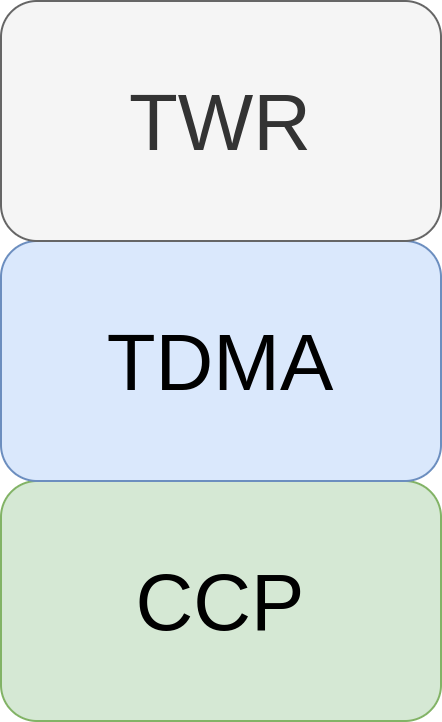
\includegraphics[width=0.6\textwidth]{ranging_layered_architecture}
            \end{center}
            \caption{Ranging layered architecture}
            \label{fig:ranging_layered_architecture}
    \end{columns}
\end{figure}
\end{frame}

\begin{frame}
    \myframetitle{RAS: CCP state diagram}
    % \begin{columns}
        % \column{0.4\textwidth}
        CCP state:
        \begin{itemize}
            \item Slave: CCP\_SLAVE
            \item Master:  CCP\_MASTER
            \item Master Request: CCP\_MASTER\_REQT
        \end{itemize}
        % \column{0.6\textwidth}
        \begin{figure}[H]
            \centering
            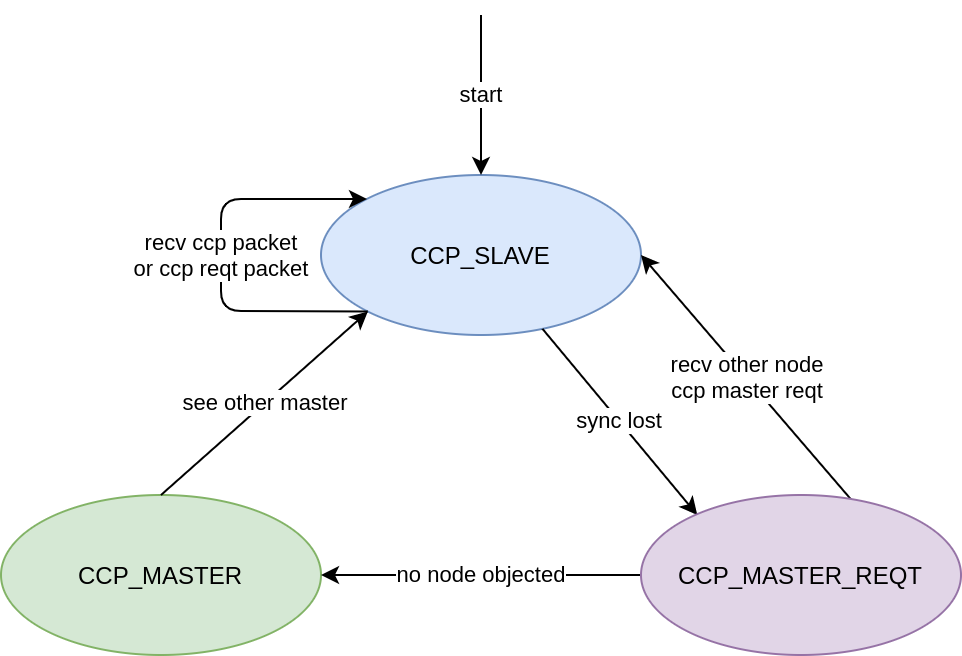
\includegraphics[width=0.6\textwidth]{ccp_state_diagram.png}
            \caption{CCP state transition diagram}
            \label{fig:CCP_state_diagram}
        \end{figure}
    % \end{columns}
\end{frame}

\begin{frame}
    \myframetitle{RAS: Slave Flowchart}
    \begin{columns}
        \column{0.5\textwidth}
        \begin{figure}[H]
            \centering
            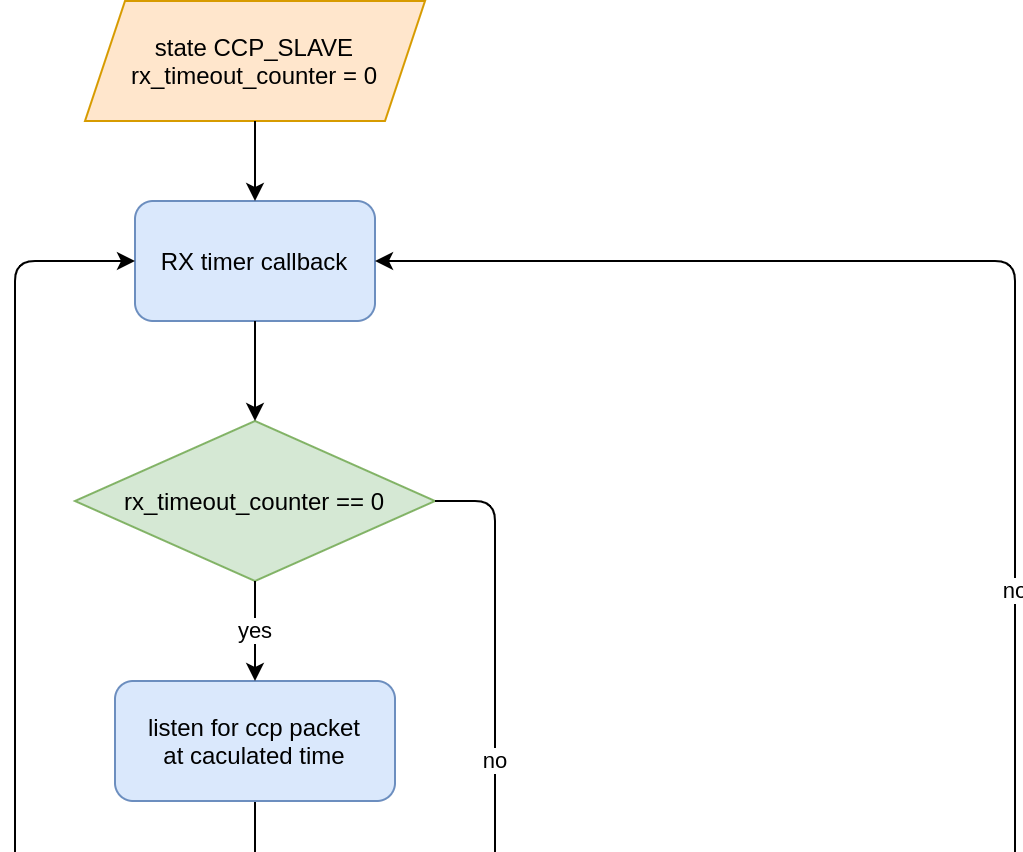
\includegraphics[width=0.9\textwidth]{ccp_slave_flowchart_01.png}
            \caption{CCP slave flow chart}
            \label{fig:ccp_slave_flow_chart}
        \end{figure}
        \column{0.5\textwidth}
        \begin{figure}[H]
            \centering
            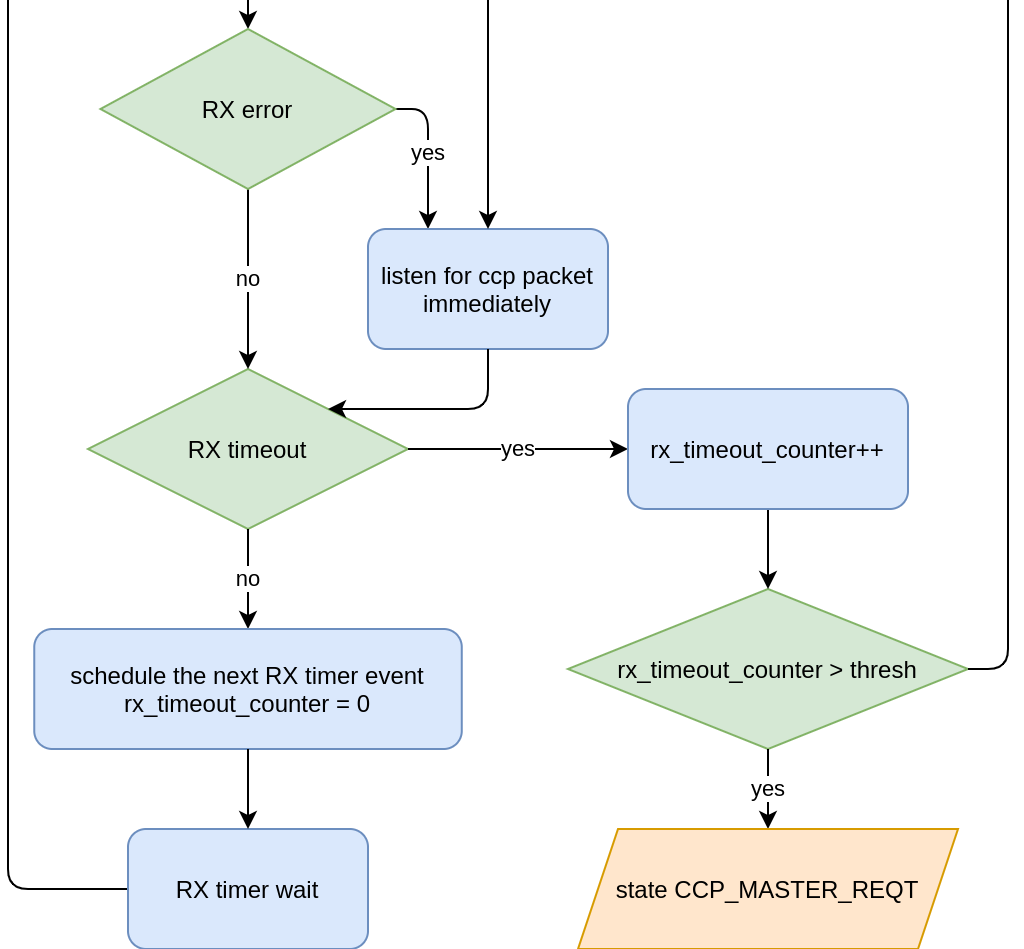
\includegraphics[width=0.9\textwidth]{ccp_slave_flowchart_02.png}
            \caption{CCP slave flow chart}
            \label{fig:ccp_slave_flow_chart}
        \end{figure}
    \end{columns}
\end{frame}

\begin{frame}
    \myframetitle{RAS: Master and Master Request Flowchart}
    \begin{columns}
        \column{0.5\textwidth}
        \begin{figure}[H]
            \centering
            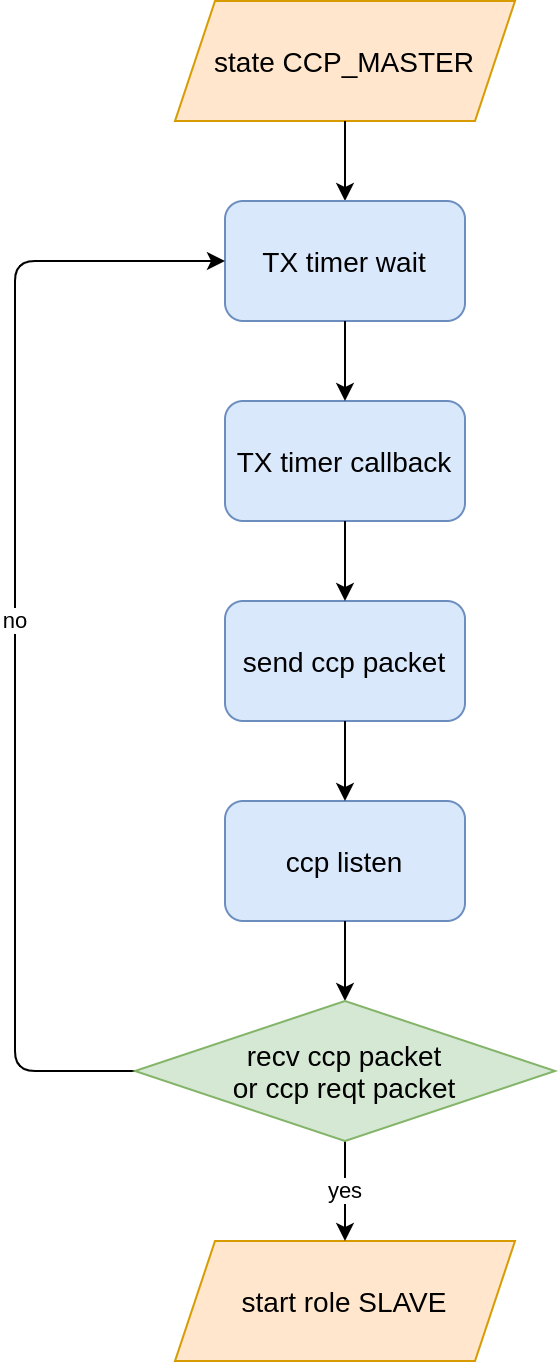
\includegraphics[width=0.45\textwidth]{ccp_master_flow_chart.png}
            \caption{CCP master flowchart}
        \end{figure}
        \column{0.5\textwidth}
        \begin{figure}[H]
            \centering
            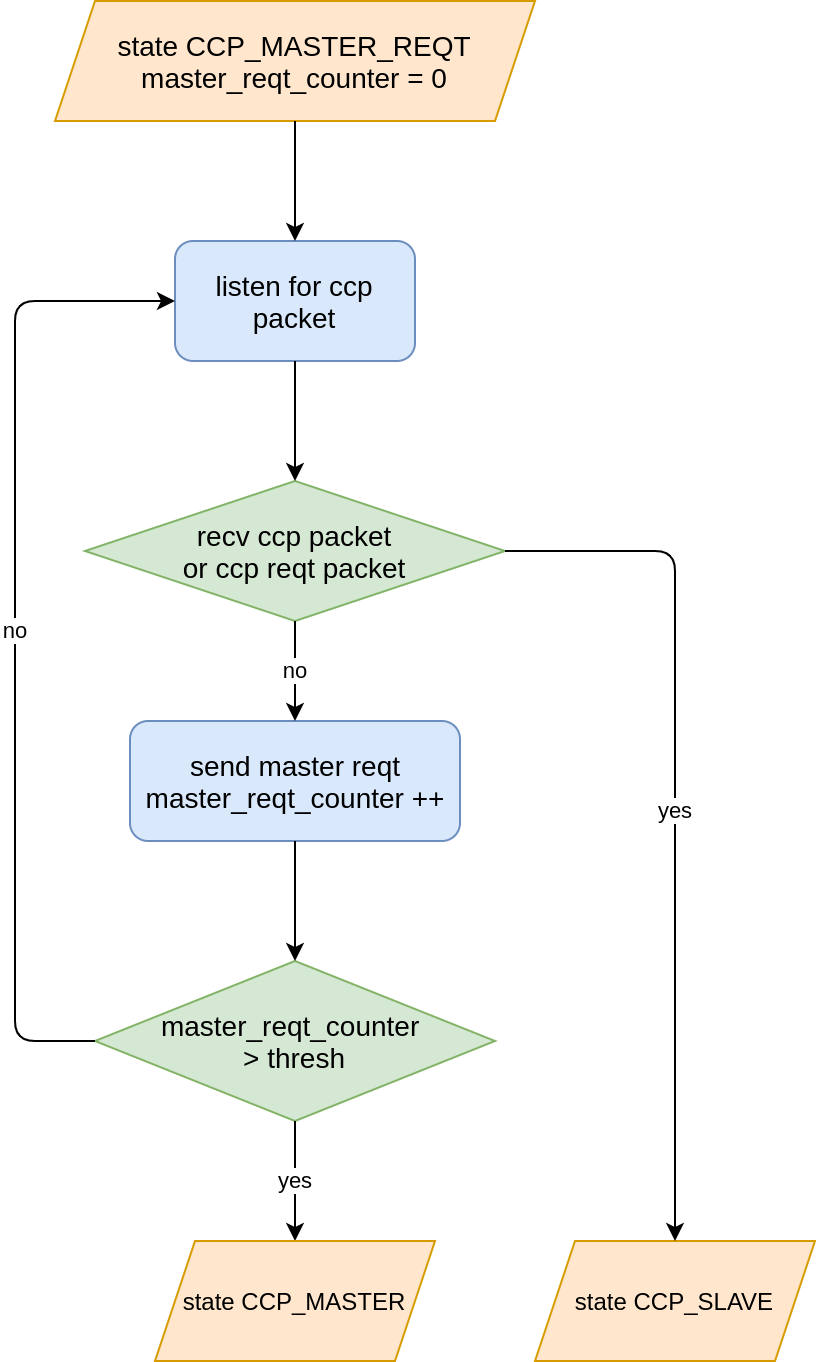
\includegraphics[width=0.65\textwidth]{ccp_master_reqt_flow_chart.png}
            \caption{CCP master request flowchart}
            \label{fig:ccp_slave_flow_chart}
        \end{figure}
    \end{columns}
\end{frame}

\begin{frame}
    \myframetitle{RSA: CCP Master Timing}
    \begin{columns}
        \column{0.4\textwidth}
        \begin{equation*}
            \begin{split}
                &t^k_m = t^{k-1}_m + \tau \\
                &ep_m = ep_l = t^k_m - T_{SHR} 
            \end{split}
        \end{equation*}
        \column{0.6\textwidth}
        \begin{equation*}
            \begin{split}
                &ep_o = t_h - f_{d2h}(t_d - t^k_m) - T_{SHR}\\
                &t_{wake up} = ep_o + \tau - T_{latency}
            \end{split}
        \end{equation*}
    \end{columns}
    \begin{figure}[H]
        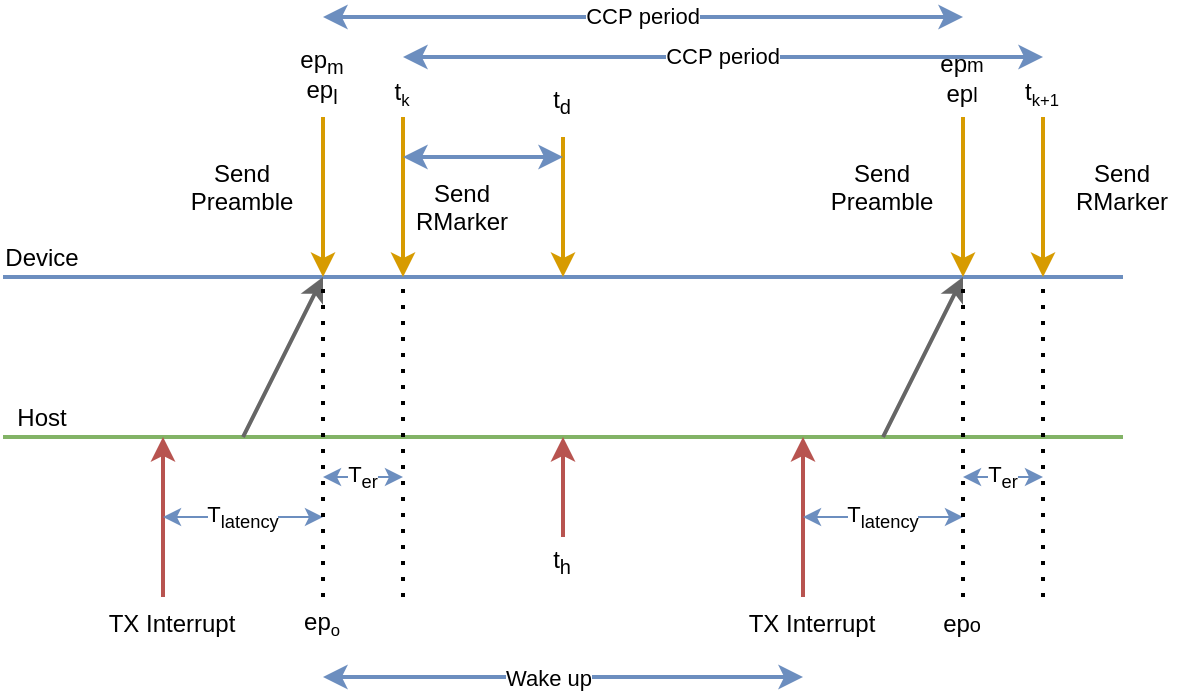
\includegraphics[width=0.75\textwidth]{ccp_timing_for_master_node.png}
        \caption{CCP master timing}
        \label{fig:interupt_latency_master}
    \end{figure}
\end{frame}

\begin{frame}
    \myframetitle{RSA: CCP Slave Timing - Message Relay}
    \begin{columns}
        \column{0.4\textwidth}
        \begin{equation*}
            \begin{split}
                & ep_m = t^k_m - T_{SHR}\\
                & ep_l = t^k_l - T_{SHR} \\
                & ep_o = t_h - f_{d2h}(t_d - t^k_l) - T_{SHR}\\
                & t_{wake up} = ep_o + \tau - T_{latency}
            \end{split}
        \end{equation*}
        \column{0.6\textwidth}
        \begin{equation*}
            \begin{split}
                &T_{hold-off} = n_{repeat}*T_{hold-off-conf} + i_{slot}*T_{ccp}\\
                &t^{k-repeat} = t^k + T_{hold-off}\\
                &\tau_{new} = \tau - T_{hold-off}
            \end{split}
        \end{equation*}
    \end{columns}
    \begin{figure}[H]
        \begin{center}
            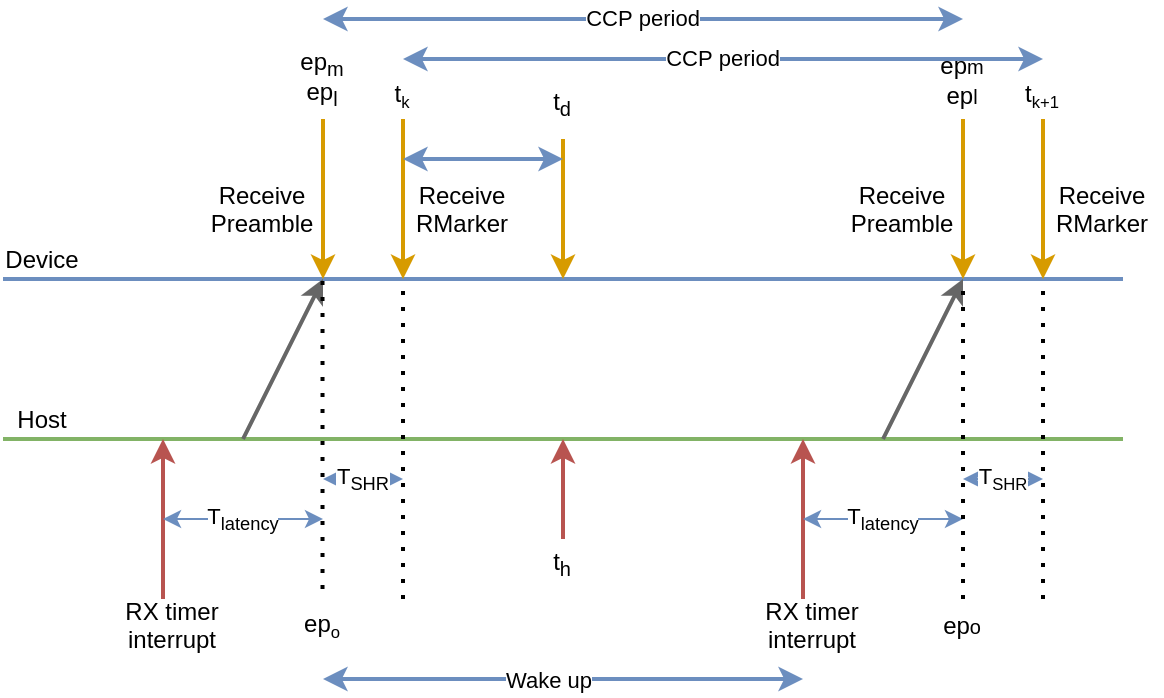
\includegraphics[width=0.65\textwidth]{ccp_timing_for_slave_node.png}
        \end{center}
        \caption{CCP slave timing}
        \label{fig:ccp_timing_for_slave_node}
    \end{figure}
\end{frame}

\begin{frame}
    \myframetitle{RSA: TDMA state diagram}
    2 TDMA states:
    \begin{itemize}
        \item TDMA\_REQT
        \item TDMA\_JOINTED
    \end{itemize}
    \begin{columns}
        \column{0.75\textwidth}
        \begin{figure}[H]
            \begin{center}
                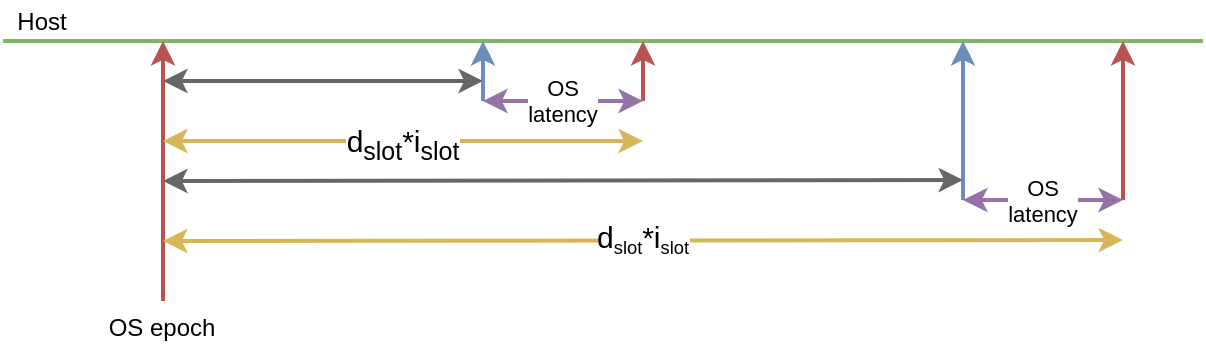
\includegraphics[width=1\textwidth]{tdma_timing.png}
            \end{center}
            \caption{TDMA timing}
            \label{fig:tdma_timing}
        \end{figure}
        \column{0.25\textwidth}
        \begin{figure}[H]
            \begin{center}
                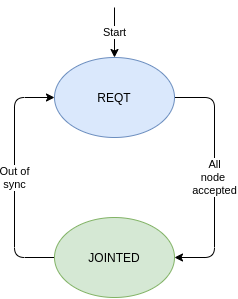
\includegraphics[width=0.9\textwidth]{tdma_state_diagram.png}
            \end{center}
            \caption{TDMA state diagram}
            \label{fig:tdma_state_diagram}
        \end{figure}
    \end{columns}
    \begin{equation*}
        t_{slot-wake-up} = d_{slot}*i_{slot} - T_{os-latency}
    \end{equation*}
\end{frame}

\begin{frame}
    \myframetitle{RSA: TDMA REQT Flowchart}
    \begin{columns}
        \column{0.5\textwidth}
        \begin{figure}[H]
            \centering
            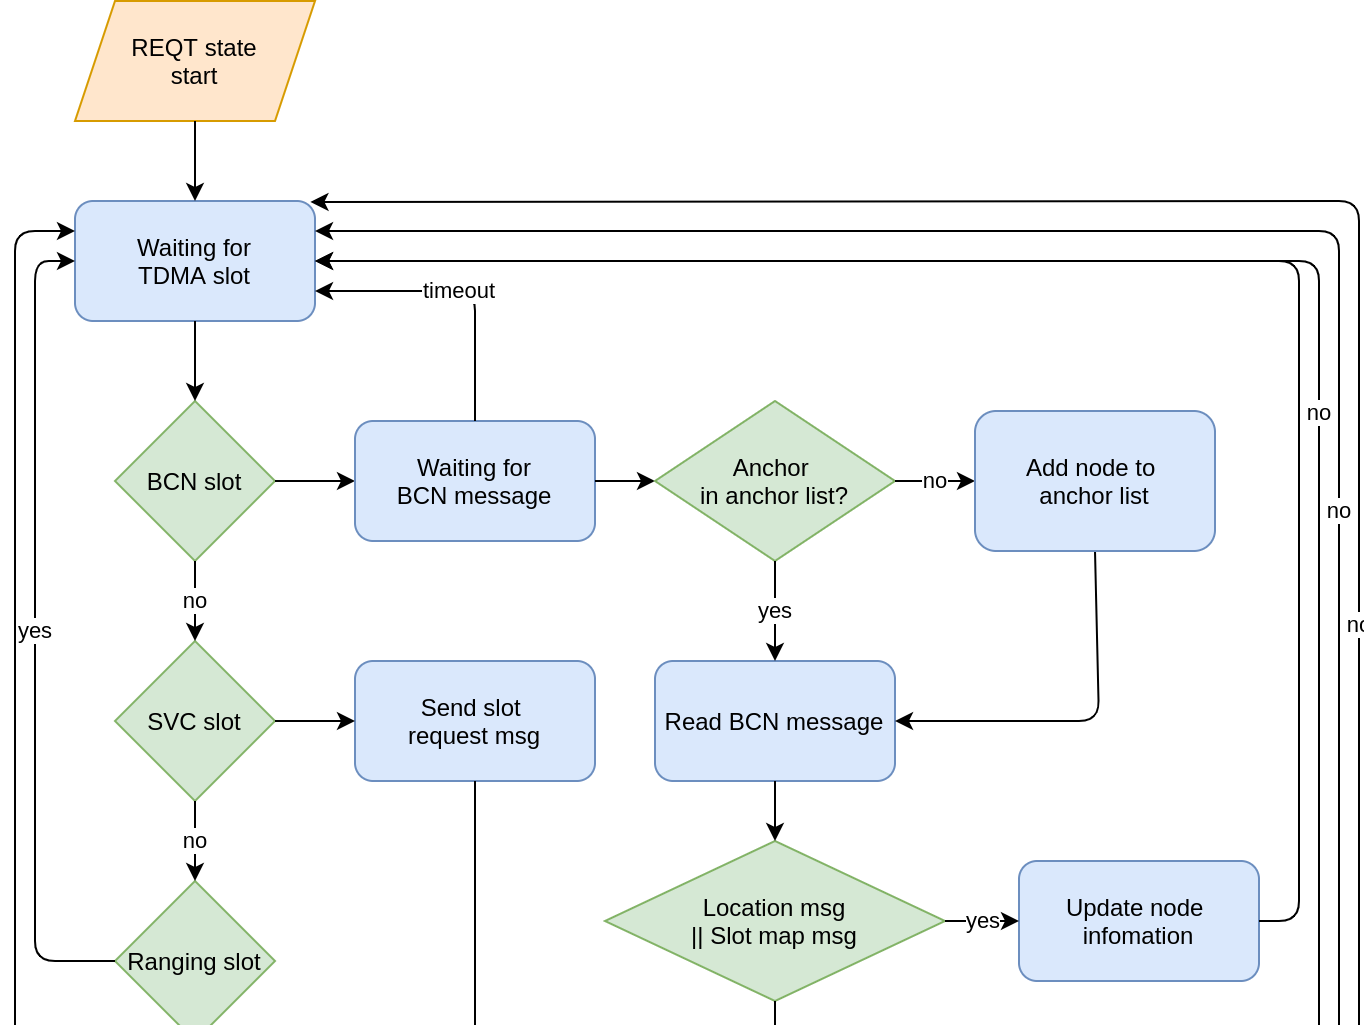
\includegraphics[width=1\textwidth]{TDMA_REQT_flowchart_01.png}
            \caption{REQT state flowchart}
        \end{figure}
        \column{0.5\textwidth}
        \begin{figure}[H]
            \centering
            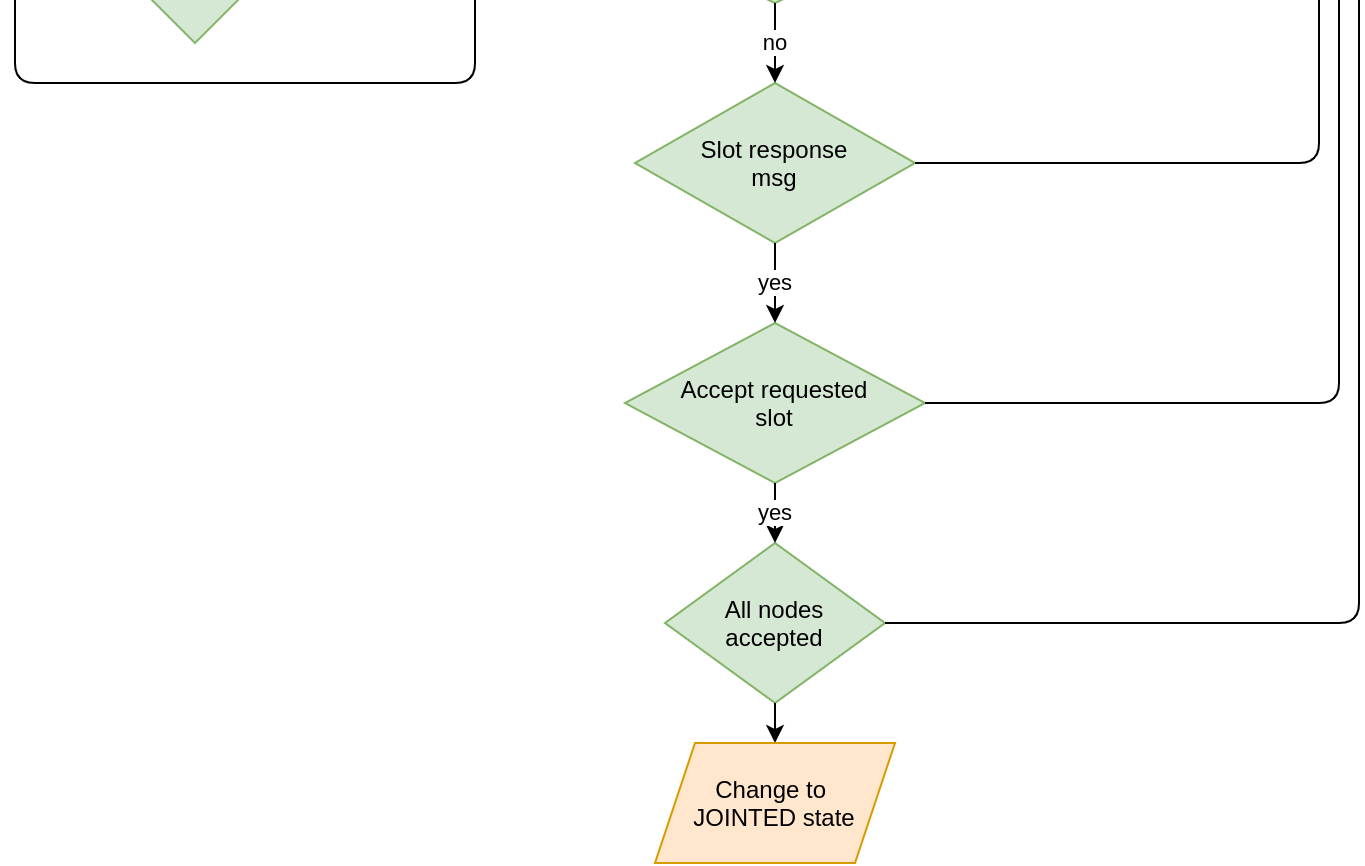
\includegraphics[width=1\textwidth]{TDMA_REQT_flowchart_02.png}
            \caption{REQT state flowchart}
        \end{figure}
    \end{columns}
\end{frame}

\begin{frame}
    \myframetitle{RSA: TDMA JOINTED Flowchart}
    \begin{columns}
        \column{0.5\textwidth}
        \begin{figure}[H]
            \centering
            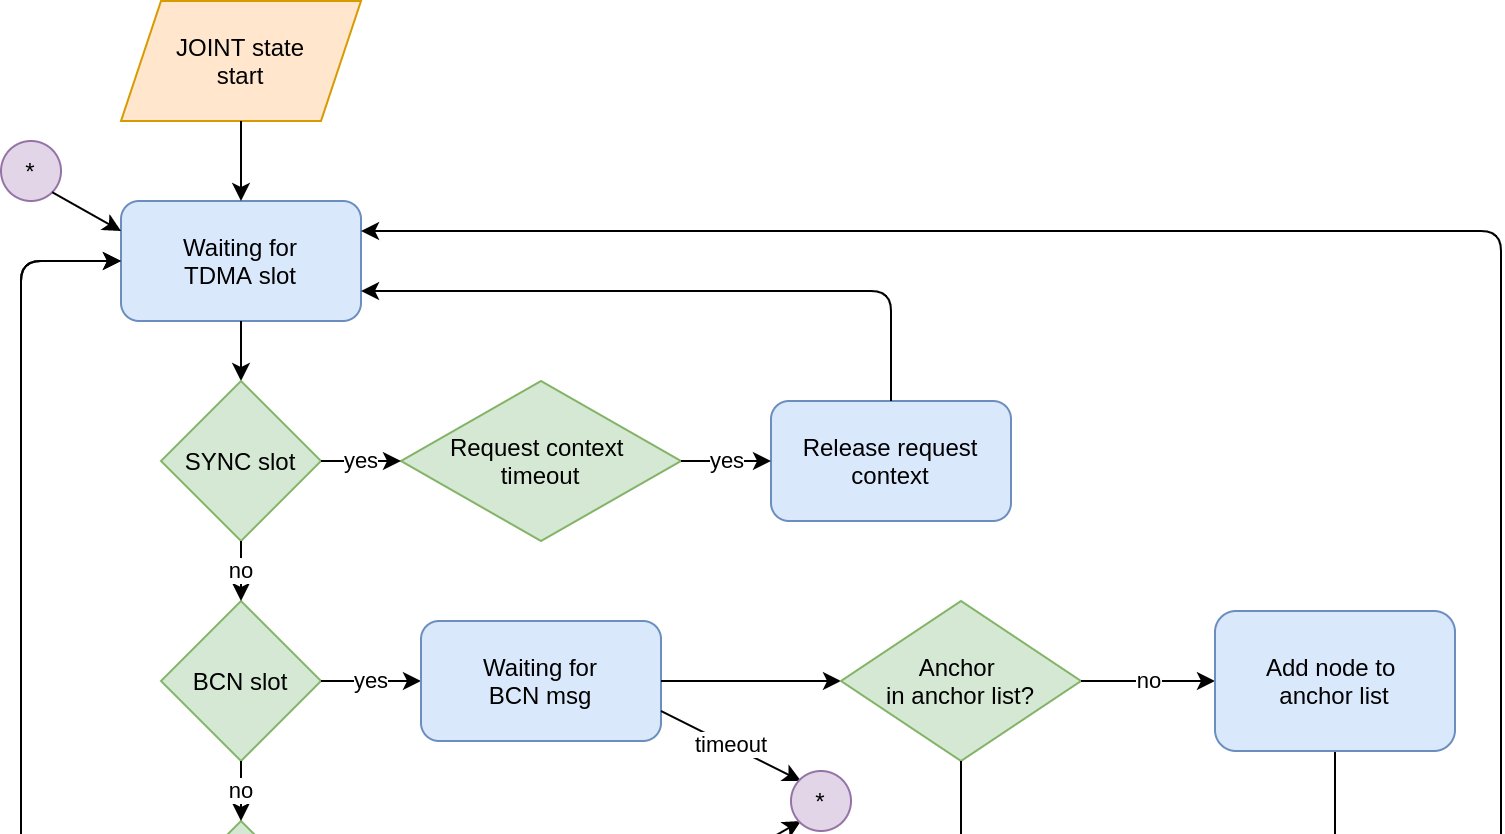
\includegraphics[width=1\textwidth]{TDMA_JOINTED_state_flowchart_01.png}
            \caption{JOINTED state flowchart}
        \end{figure}
        \column{0.5\textwidth}
        \begin{figure}[H]
            \centering
            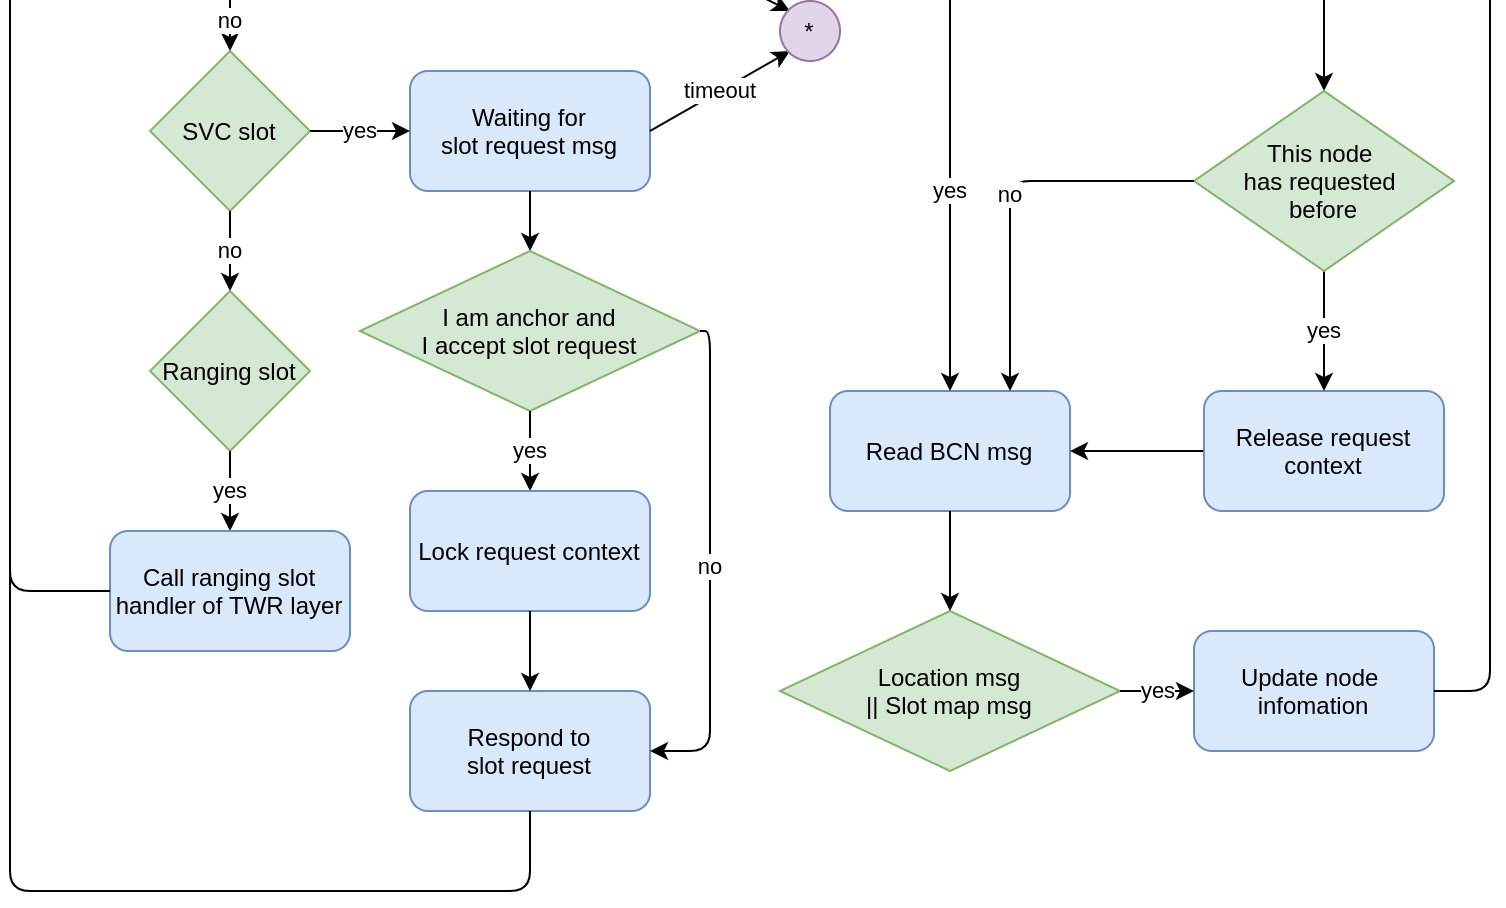
\includegraphics[width=1\textwidth]{TDMA_JOINTED_state_flowchart_02.png}
            \caption{JOINTED state flowchart}
        \end{figure}
    \end{columns}
\end{frame}

\begin{frame}
    \myframetitle{RSA: Two-Way Ranging Flowchart}
    \begin{columns}
        \column{0.5\textwidth}
        \begin{figure}[H]
            \centering
            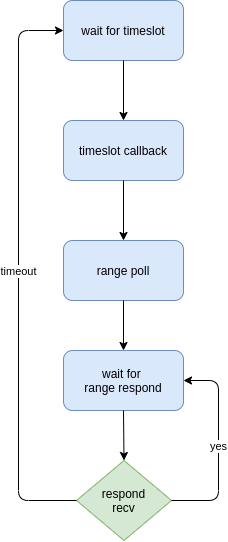
\includegraphics[height=0.75\textheight]{twr_initiator.png}
            \caption{TWR initiator flow chart}
        \end{figure}
        \column{0.5\textwidth}
        \begin{figure}[H]
            \centering
            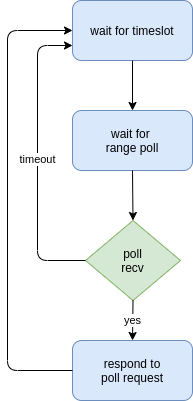
\includegraphics[height=0.75\textheight]{twr_responder.png}
            \caption{TWR responder flow chart}
        \end{figure}
    \end{columns}
\end{frame}

\begin{frame}
    \myframetitle{RSA: Two-Way Ranging}
    \begin{equation*}
        \begin{split}
            & tof = \frac{1}{2} ((t_{resp} - t_{reqt}) - (t_{trans} - t_{recp})) \\
            & T_{hold-off} = T_{hold-off-conf} + i_{slot}(T_{guard} + T_{response-frame})
        \end{split}
    \end{equation*}
    \begin{columns}
        \column{0.5\textwidth}
        \begin{figure}[H]
            \centering
            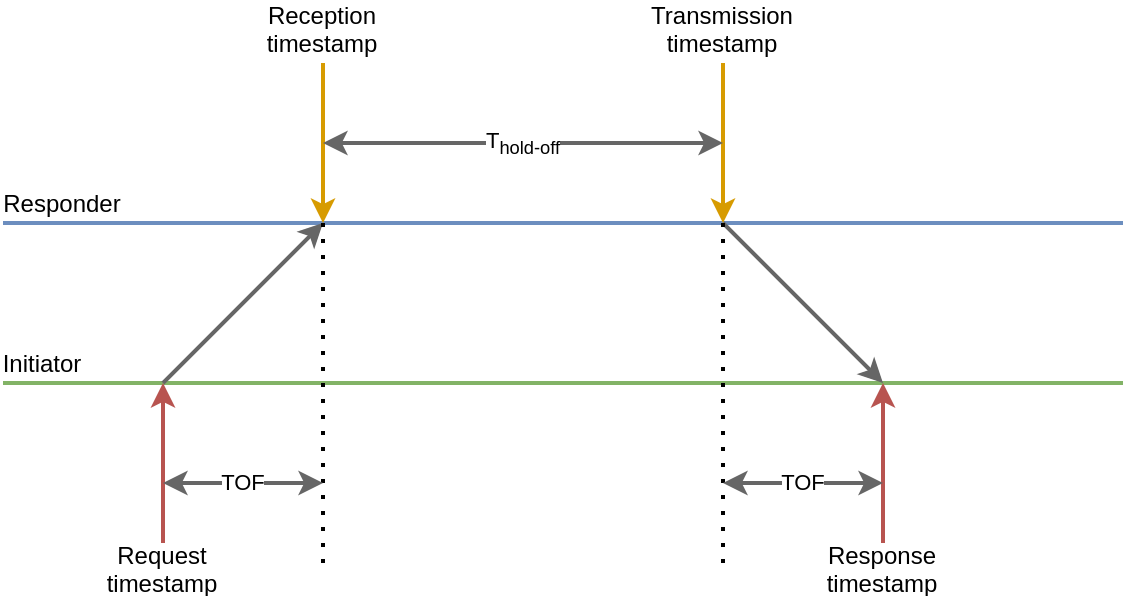
\includegraphics[width=1\textwidth]{twr_timing.png}
            \caption{Two way ranging timing}
        \end{figure}
        \column{0.5\textwidth}
        \begin{figure}[H]
            \centering
            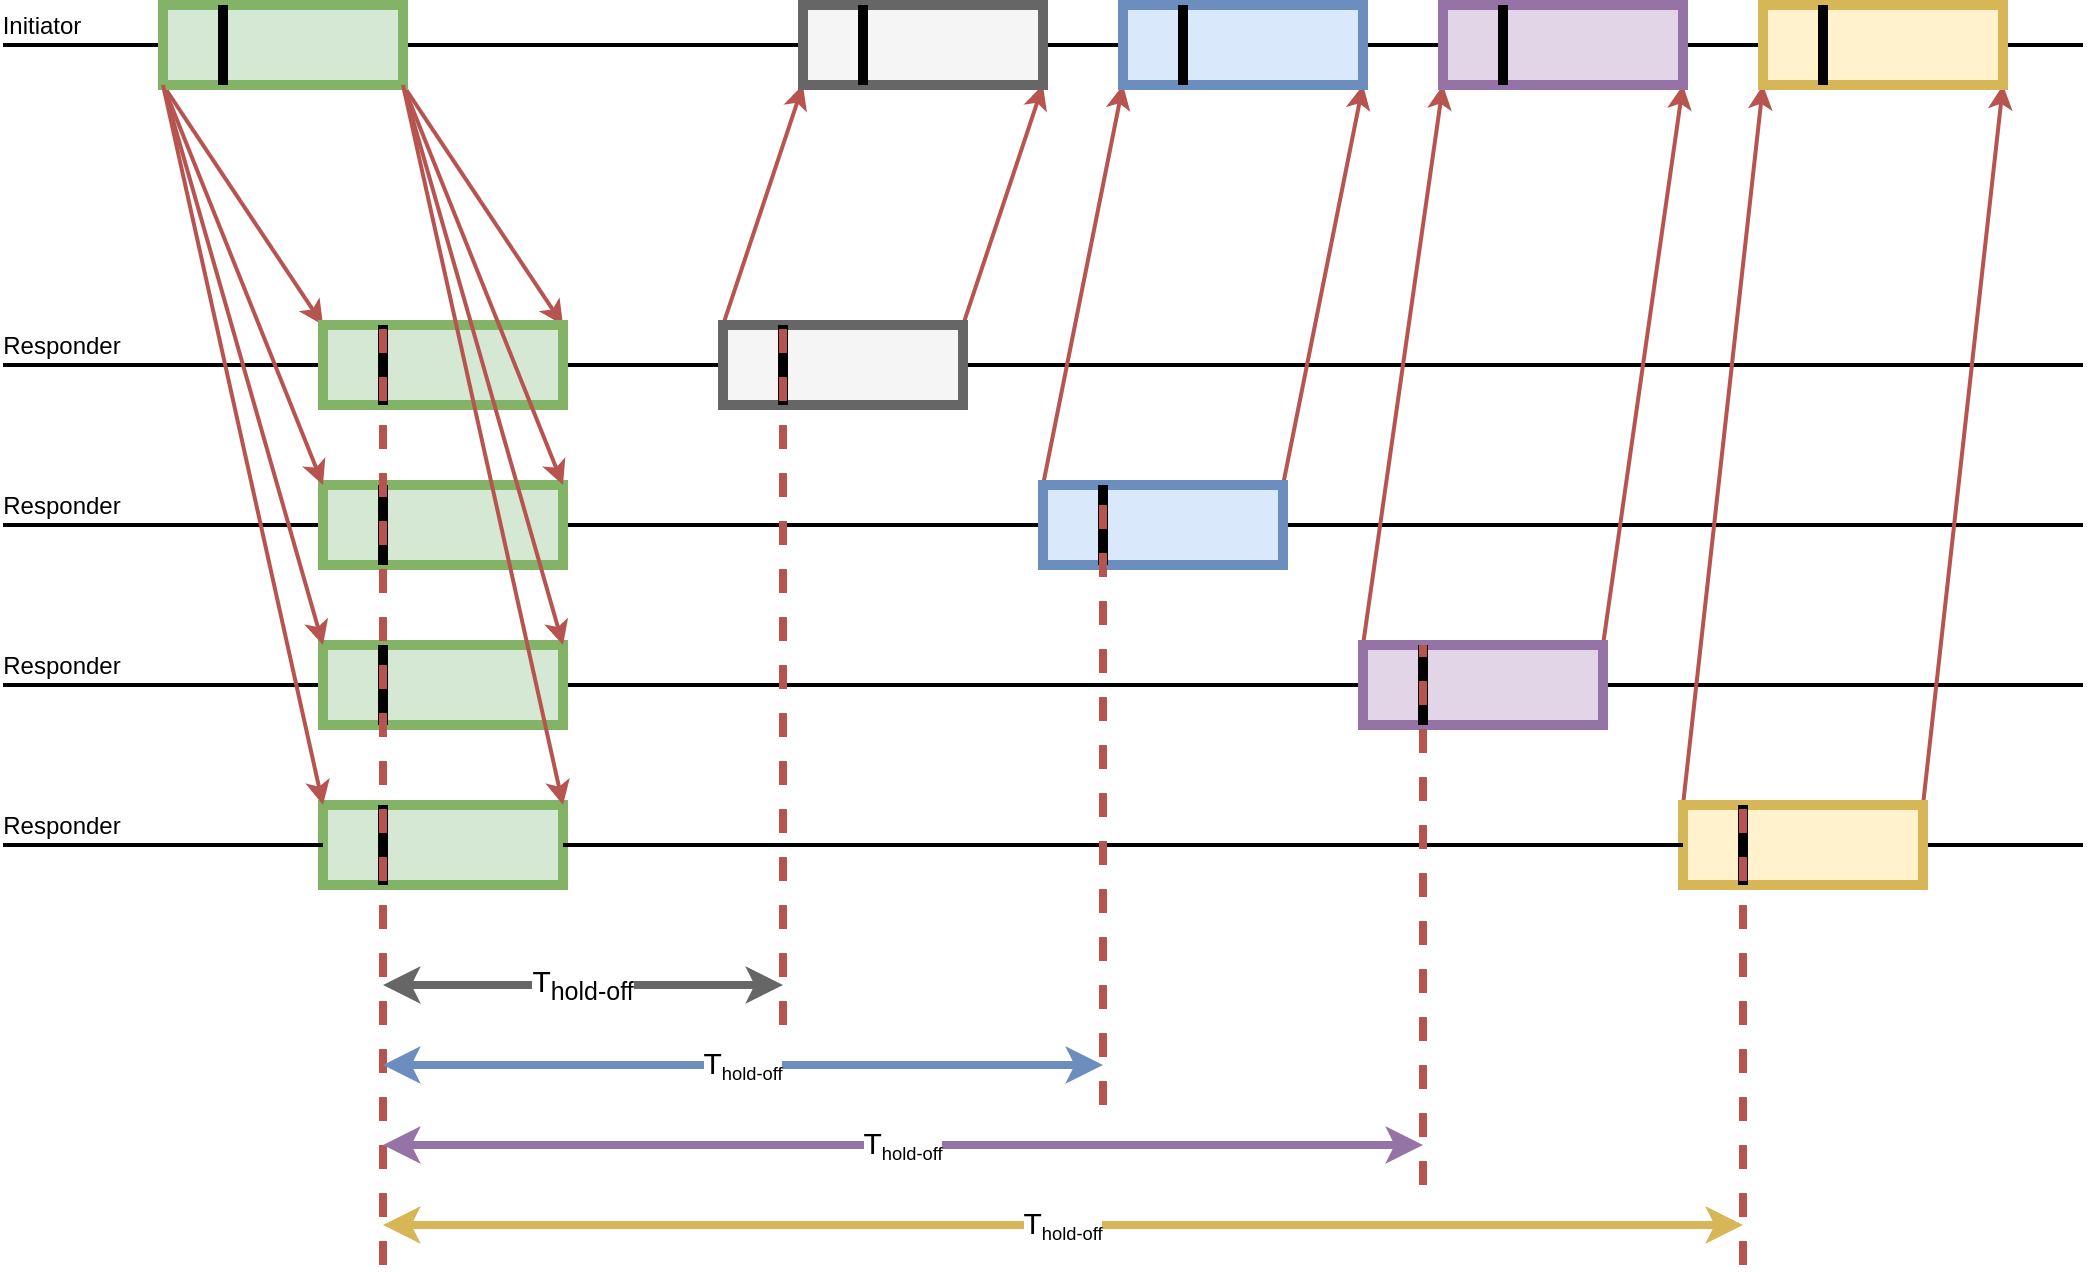
\includegraphics[width=1\textwidth]{single_sided_two_way_nranging.png}
        \caption{Single-sided two-way n ranging}
        \end{figure}
    \end{columns}
\end{frame}

\begin{frame}
    \myframetitle{RSA: Wireshark}
    \begin{figure}[H]
        \centering
        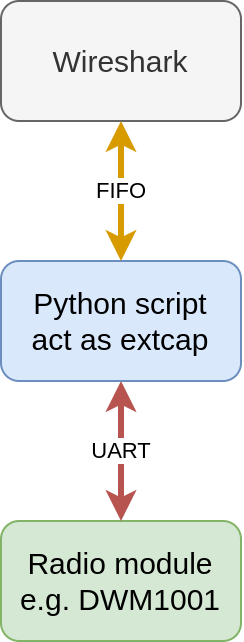
\includegraphics[width=0.6\textwidth]{extcap_802_15_4.png}
    \end{figure}
    \begin{columns}
        \column{0.5\textwidth}
        \begin{figure}[H]
            \centering
            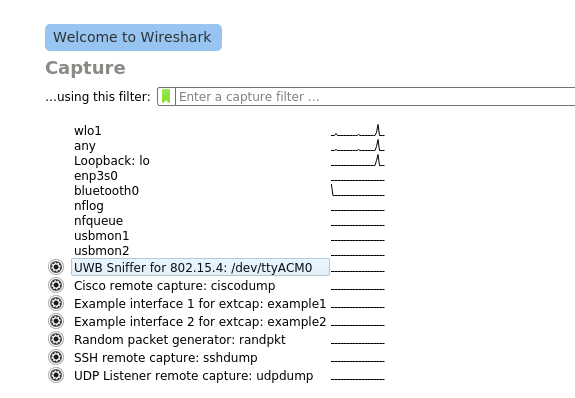
\includegraphics[width=1\textwidth]{wireshark_interface.png}
        \end{figure}
        \column{0.5\textwidth}
        \begin{figure}[H]
            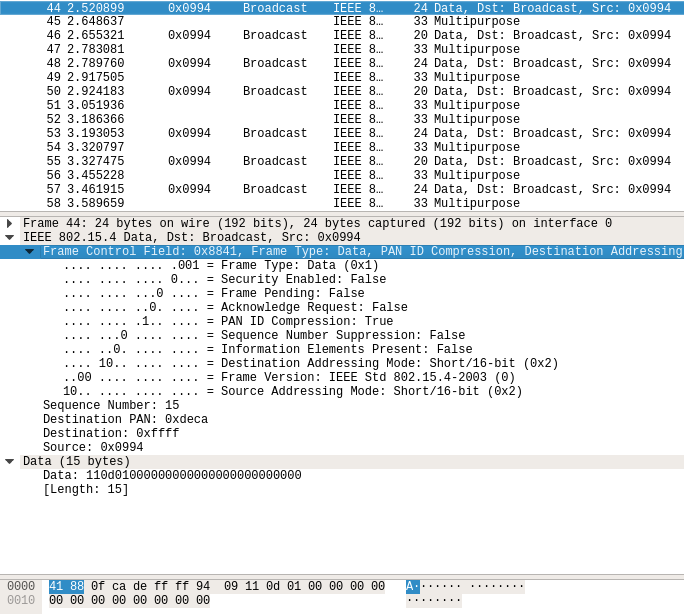
\includegraphics[width=1\textwidth]{wireshark_802_15_5_packet.png}
        \end{figure}
    \end{columns}
\end{frame}

\section{Bluetooth Mesh}

\begin{frame}
    \myframetitle{Bluetooth Mesh: Architecture}
    Terminology:
    \begin{itemize}
        \item Network: network addresses, network keys
        \item Provisioning: devices and nodes
        \item Address: unicast address, virtual address, group address
        \item Element: primary  element + additional secondary elements
        \item Model: basic functionality of a element
    \end{itemize}
    \begin{columns}
        \column{0.7\textwidth}
        \begin{figure}[H]
            \centering
            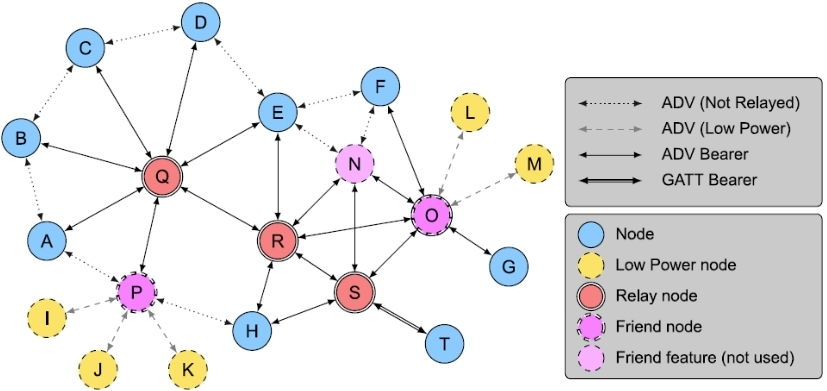
\includegraphics[width=0.9\textwidth]{mesh_topology.jpg}
            \caption{Mesh topology}
        \end{figure}
        \column{0.3\textwidth}
        \begin{figure}[H]
            \centering
            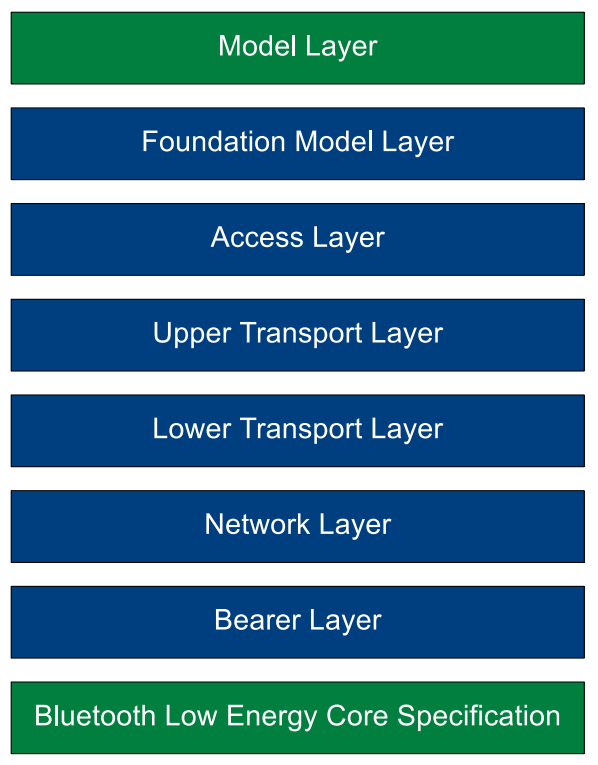
\includegraphics[width=0.9\textwidth]{ble_mesh_layered_architecture.png}
            \caption{Mesh system architecture}
        \end{figure}
    \end{columns}
\end{frame}

\begin{frame}
    \myframetitle{Bluetooth Mesh:  Best-effort Broadcast Service}
    All node publish and subscribe to a specific group address\\
    Group address: 0xC000
    \begin{figure}[H]
        \centering
        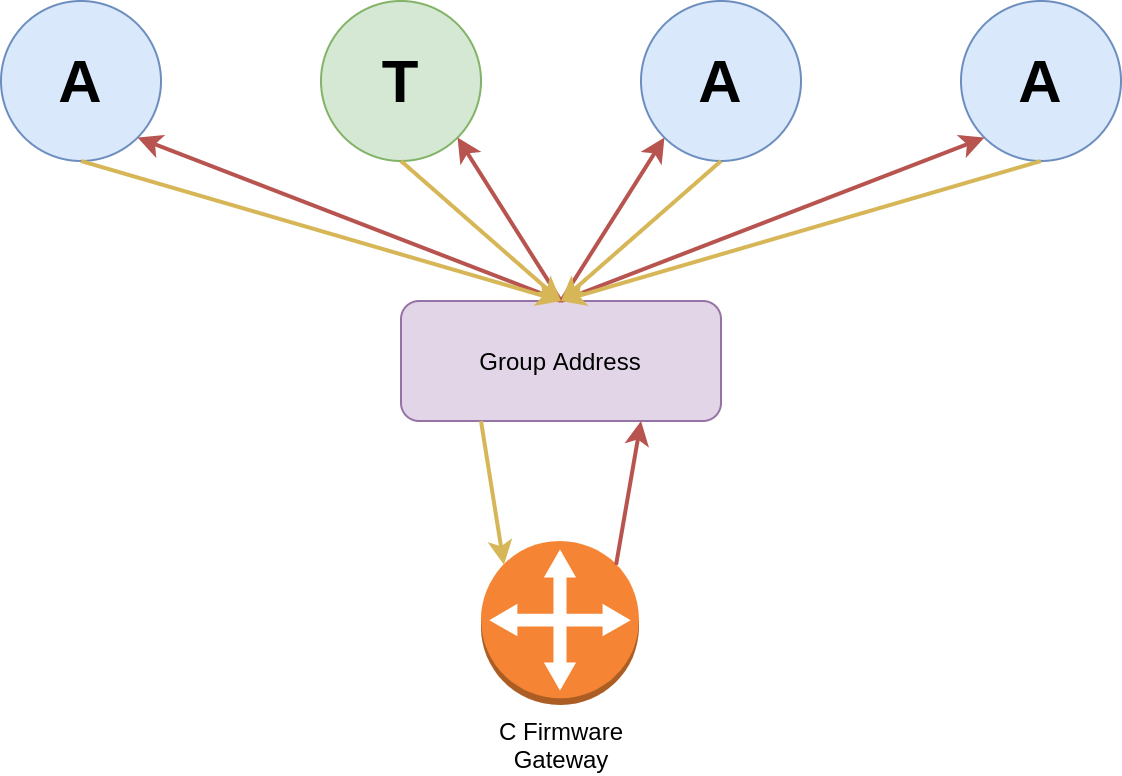
\includegraphics[width=0.6\textwidth]{ble_mesh_comunication.png}
    \end{figure}
\end{frame}

\begin{frame}
    \myframetitle{Bluetooth Mesh: nRFMesh}
    \begin{figure}[H]
        \centering
        \begin{subfigure}[b]{0.24\linewidth}
            \centering
            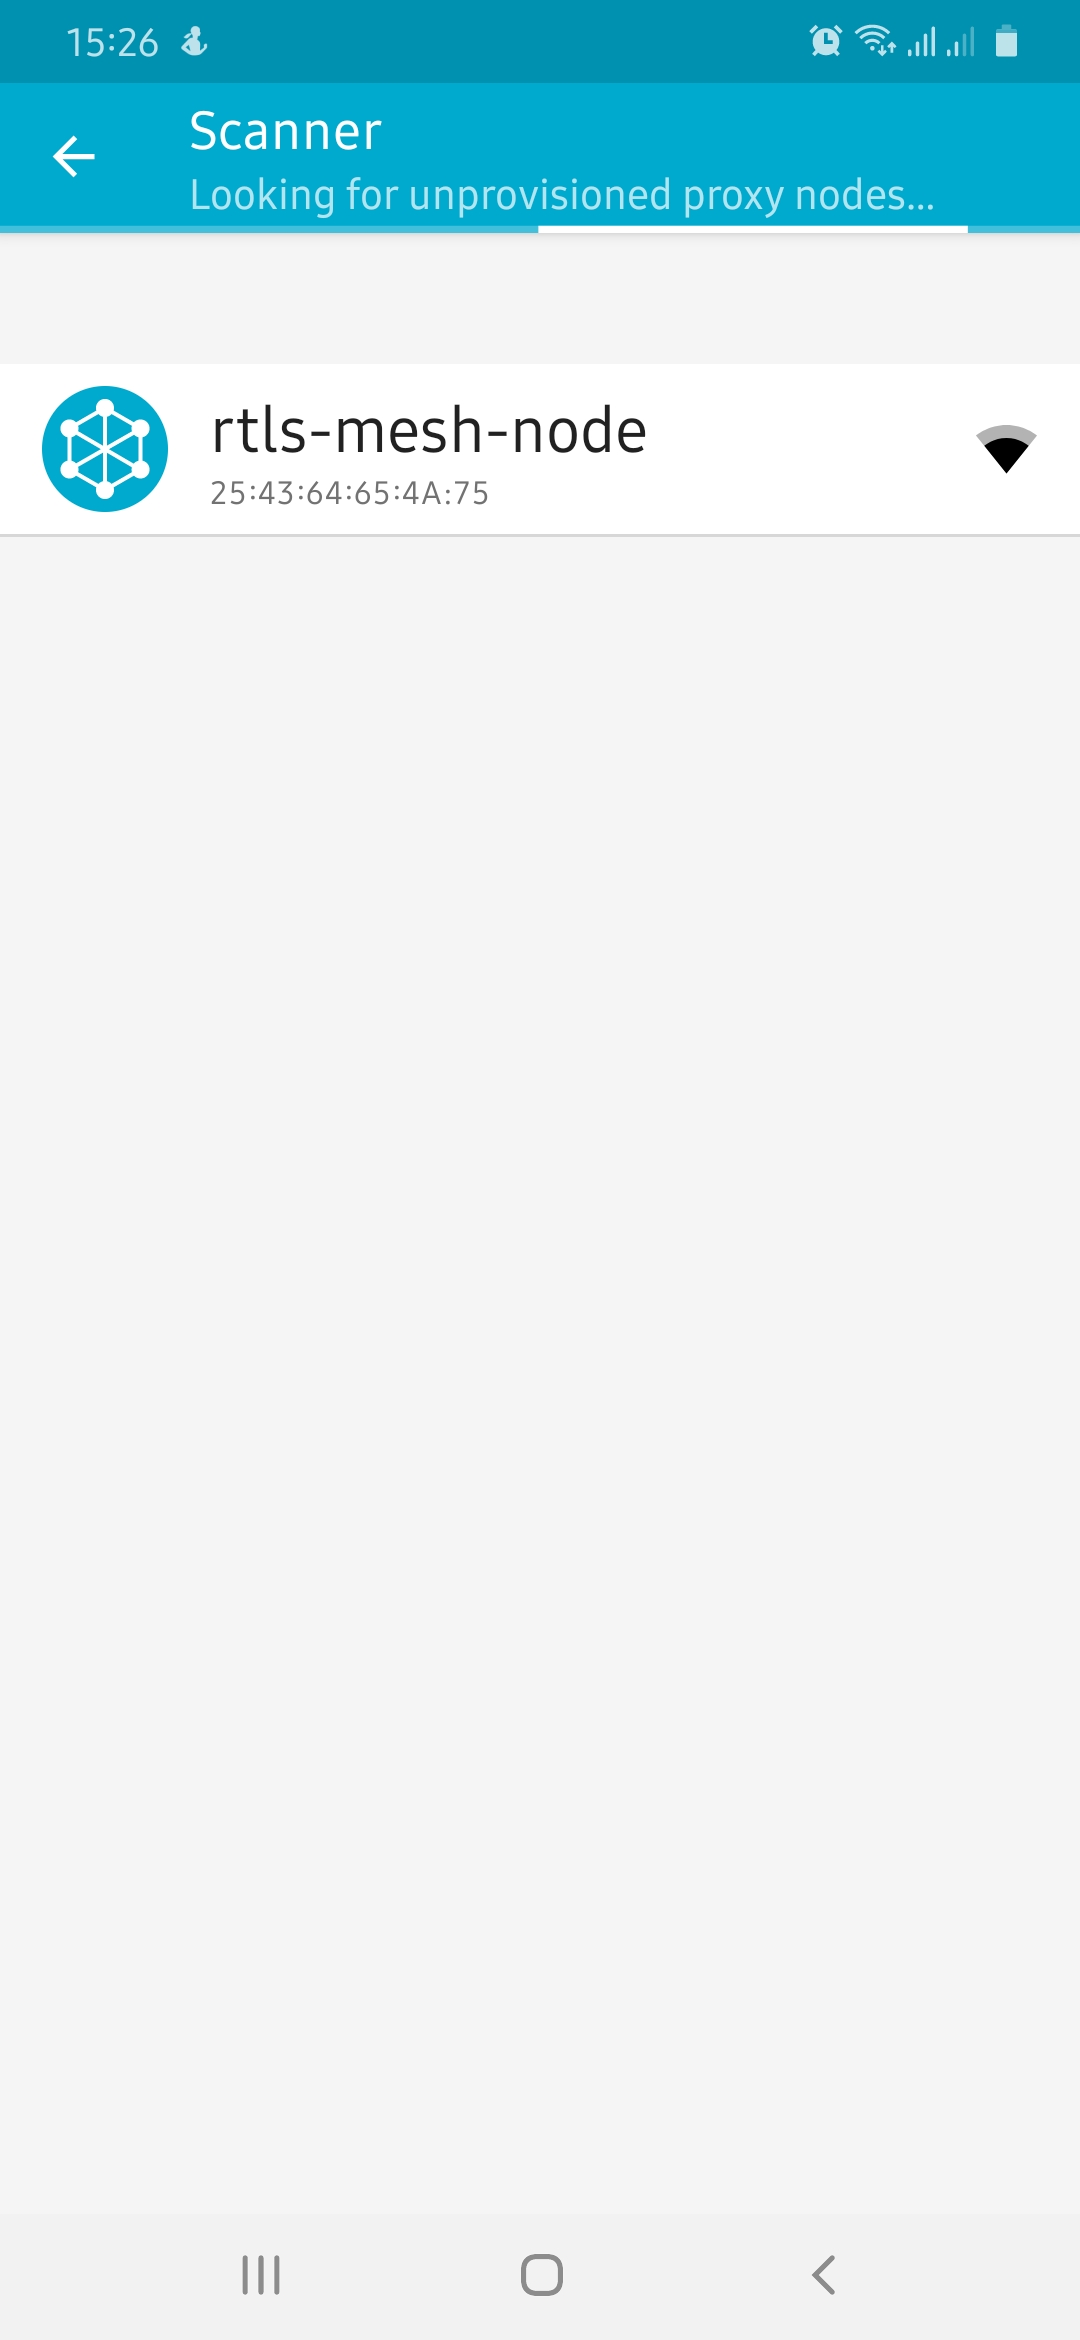
\includegraphics[width=0.9\linewidth]{nRF_Mesh_00.jpg}
            \caption{Bluetooth mesh device scan}
            \label{fig:bluetooth_mesh_device_scan}
        \end{subfigure}
        \begin{subfigure}[b]{0.24\linewidth}
            \centering
            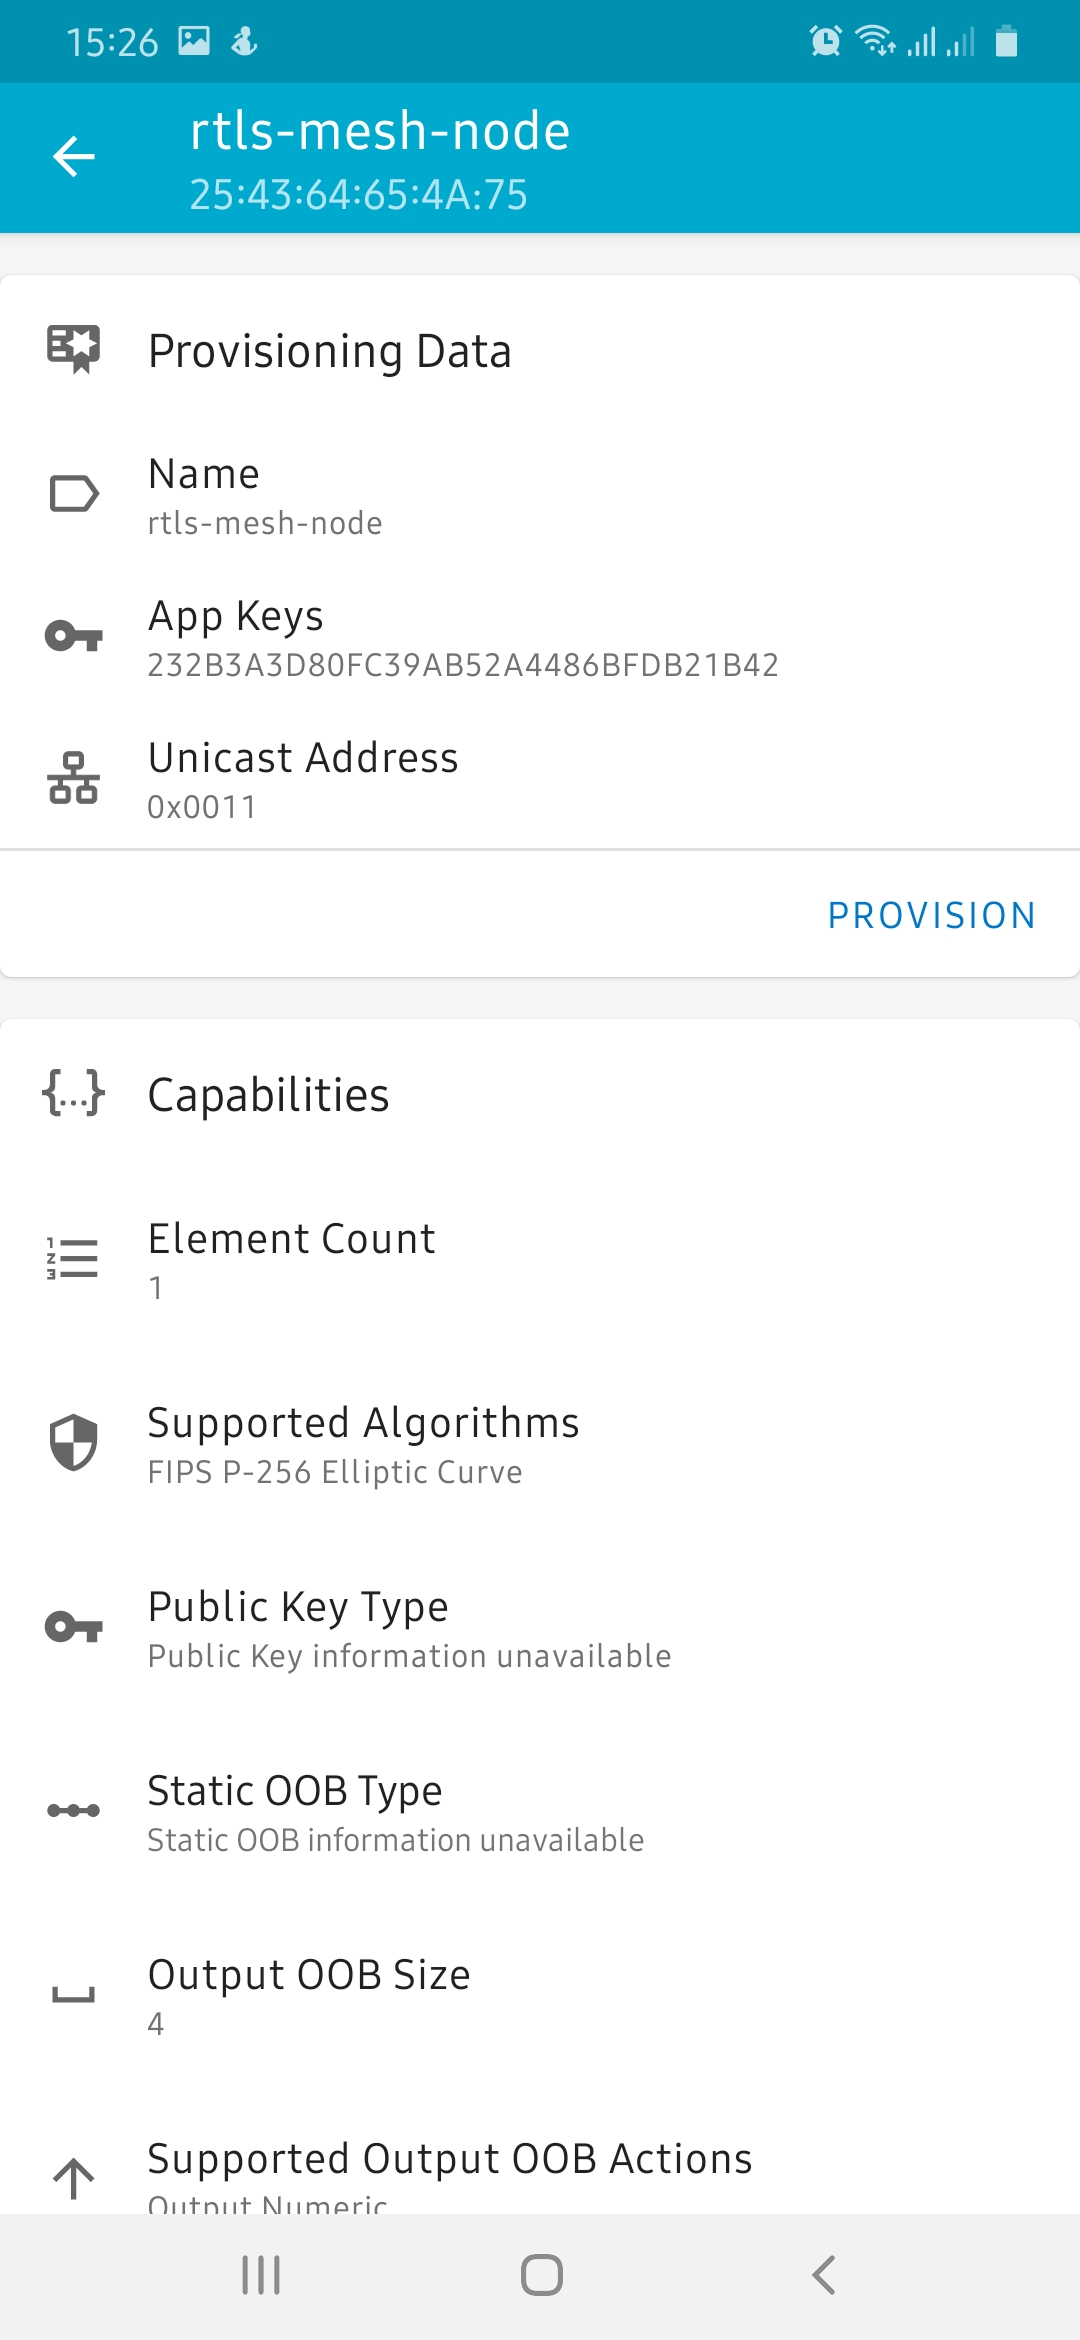
\includegraphics[width=0.9\linewidth]{nRF_Mesh_01.jpg}
            \caption{Config device address}
            \label{fig:config_device_address}
        \end{subfigure}
        \begin{subfigure}[b]{0.24\linewidth}
            \centering
            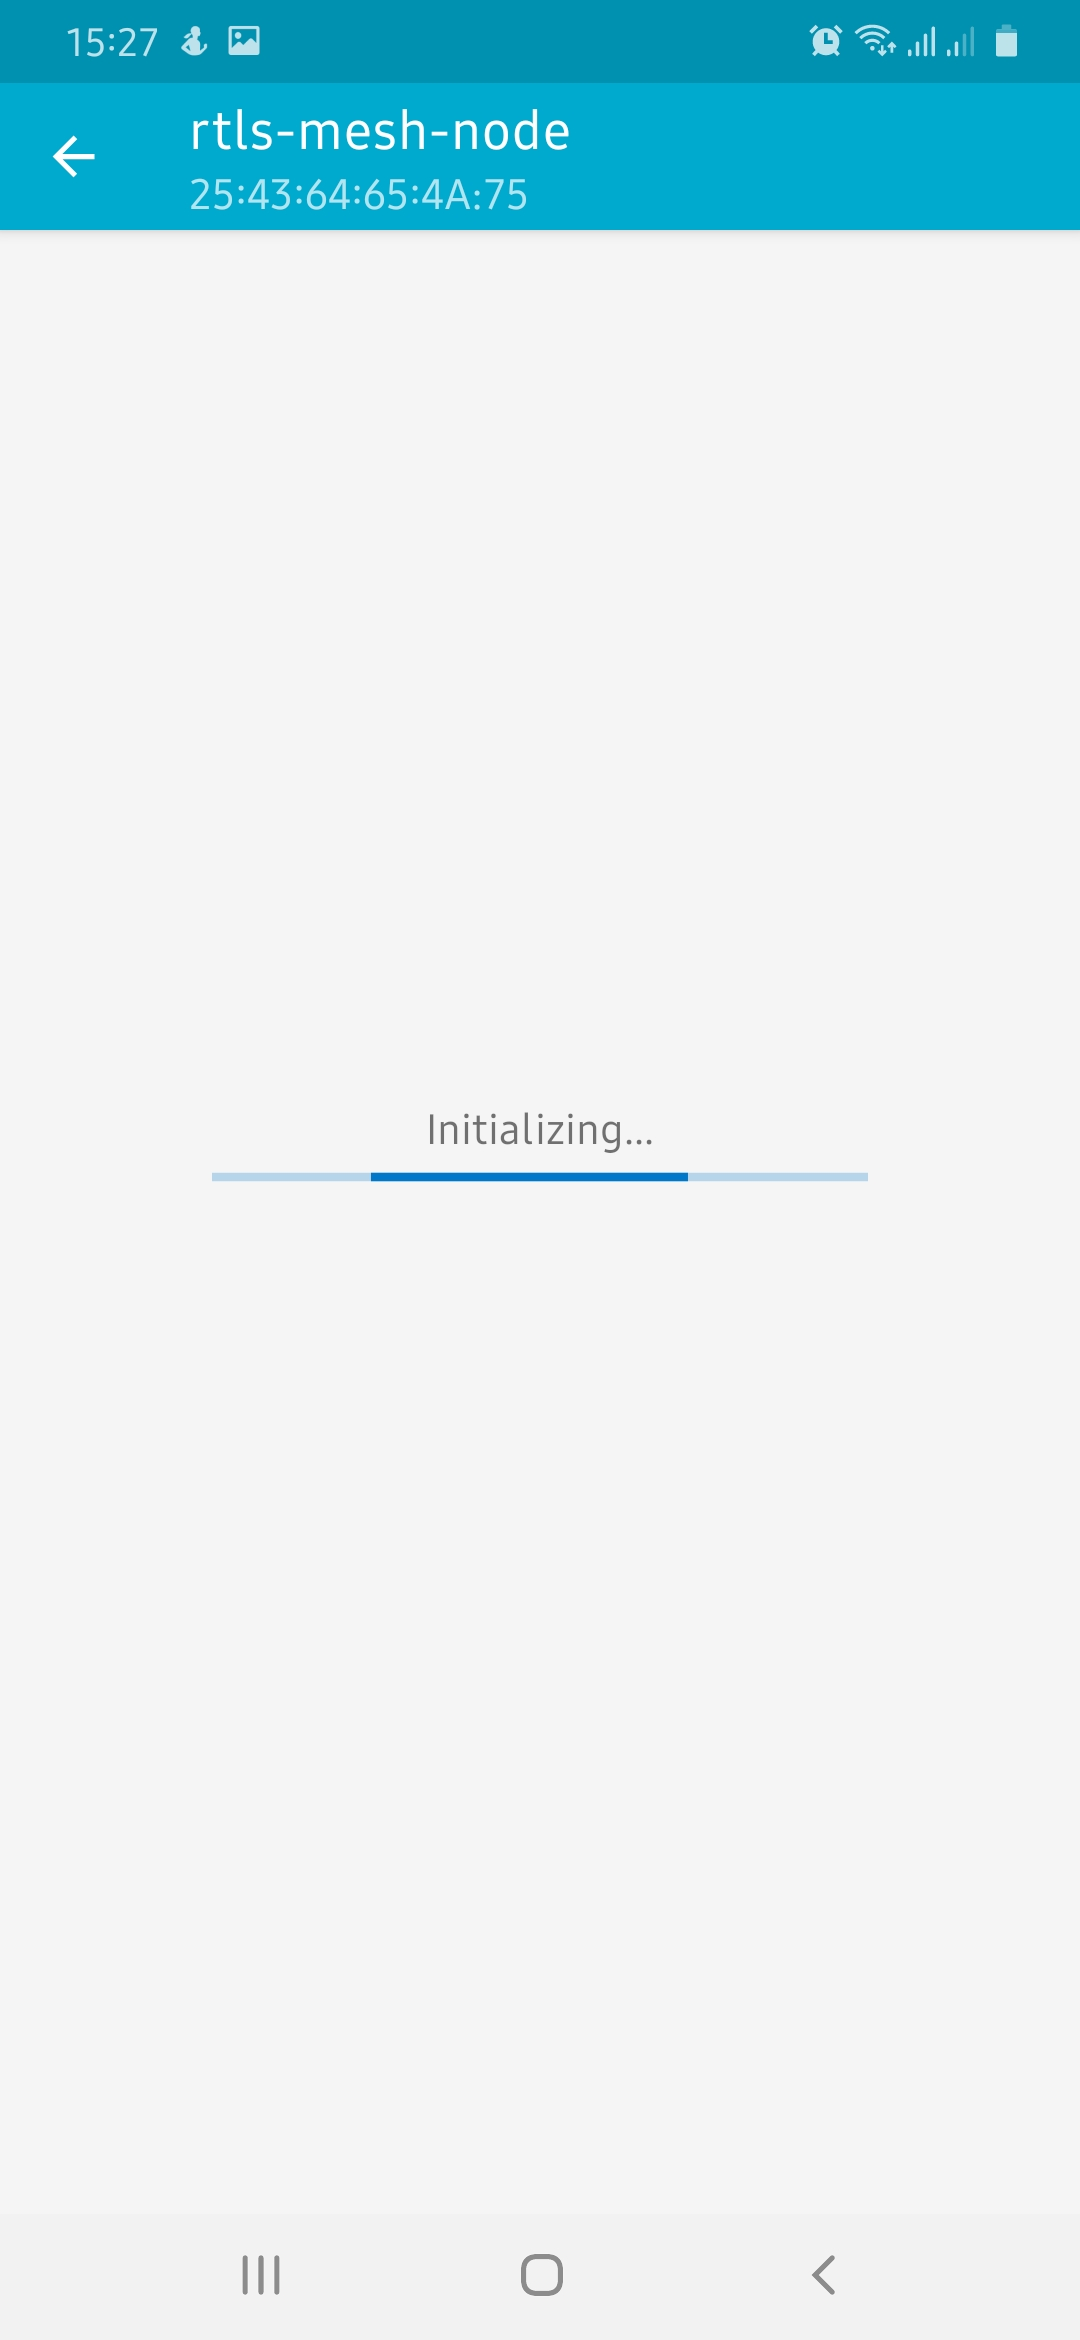
\includegraphics[width=0.9\linewidth]{nRF_Mesh_02.jpg}
            \caption{Bluetooth mesh provisioning}
        \end{subfigure}
        \begin{subfigure}[b]{0.24\linewidth}
            \centering
            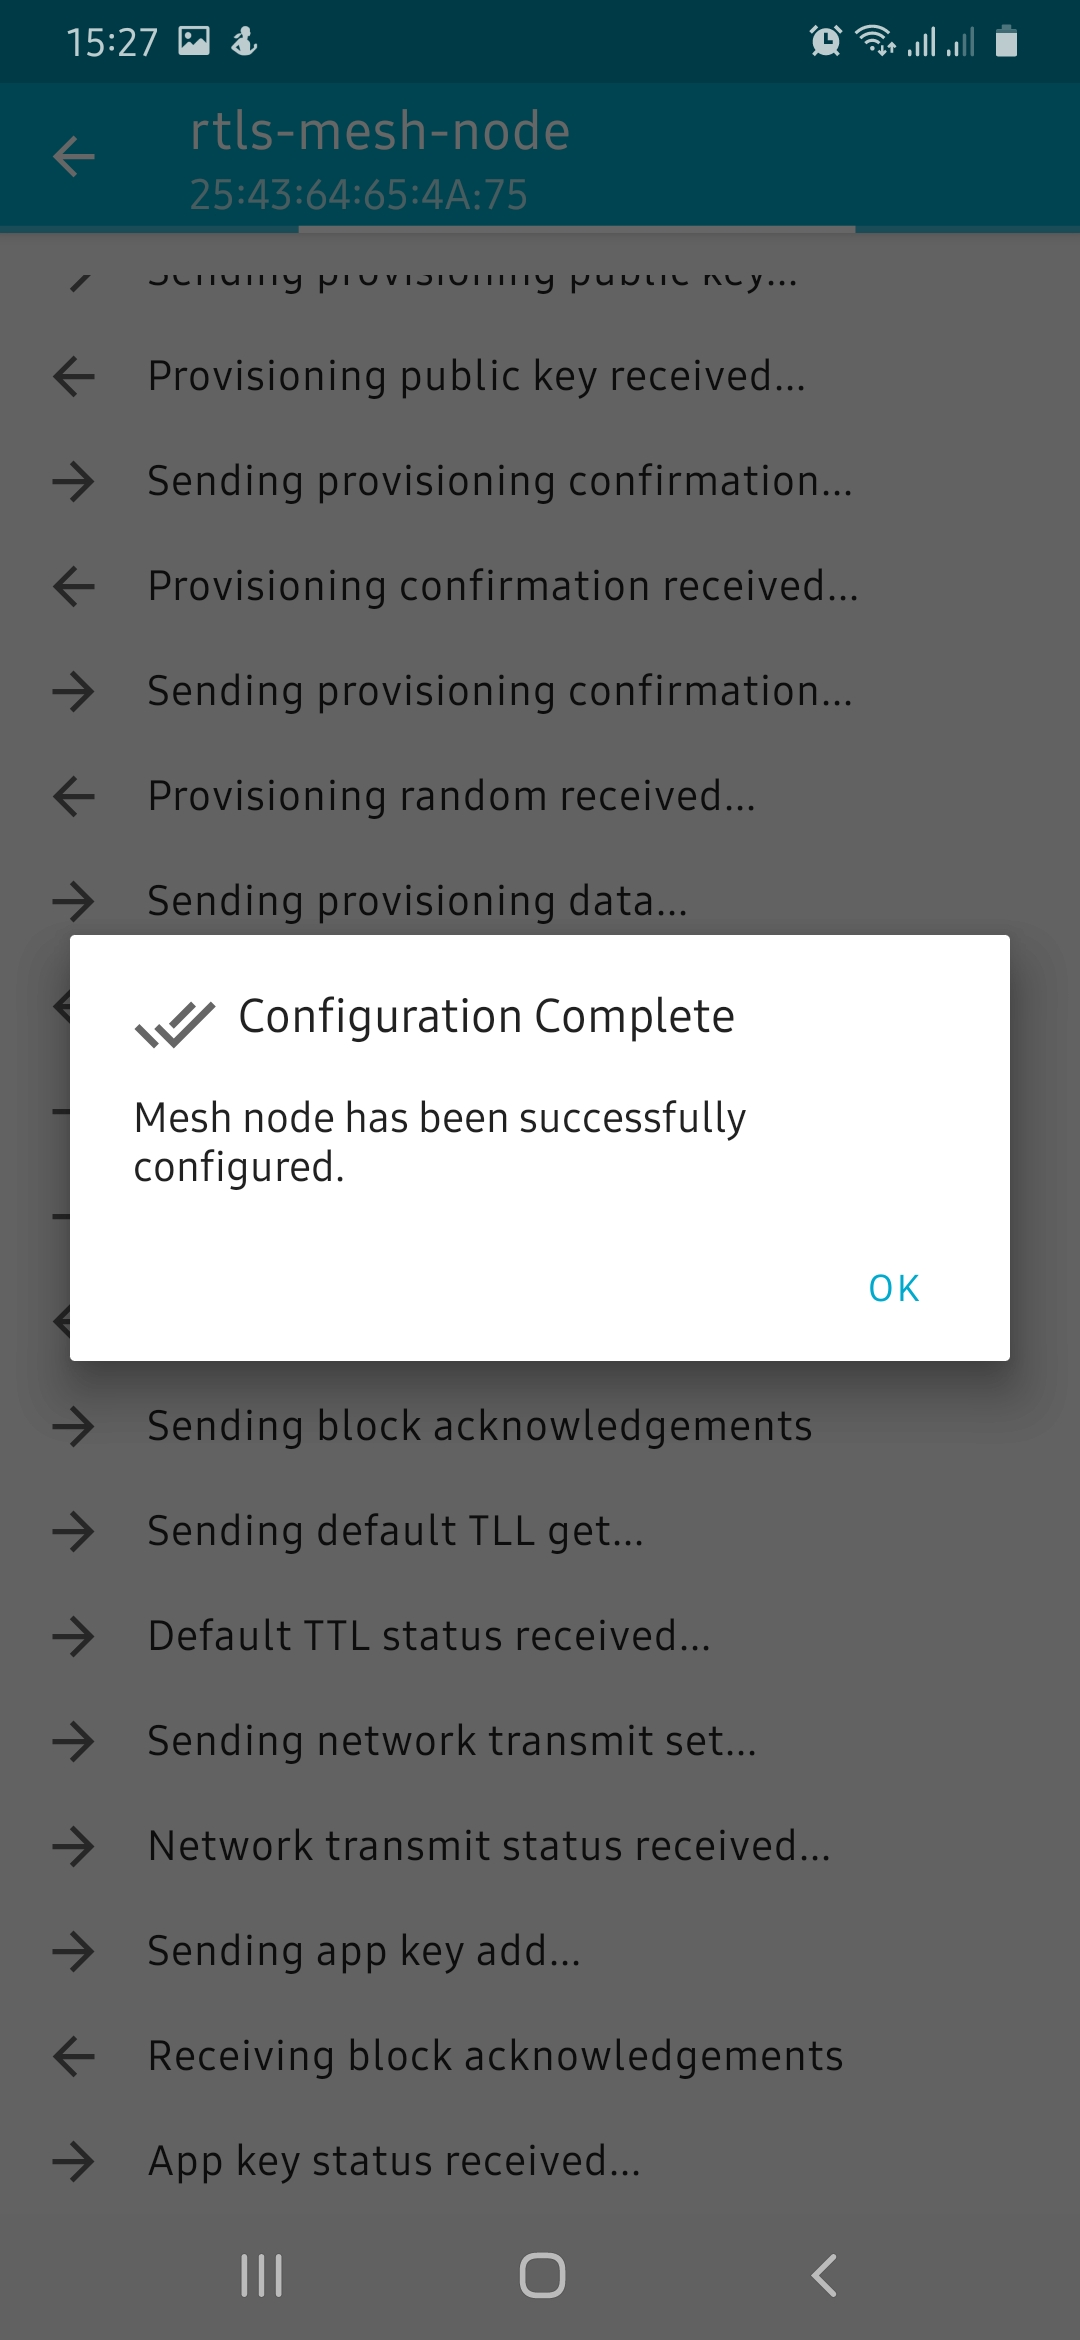
\includegraphics[width=0.9\linewidth]{nRF_Mesh_03.jpg}
            \caption{Device provision complete}
        \end{subfigure}
    \end{figure}
\end{frame}

\begin{frame}
    \myframetitle{Bluetooth Mesh: nRFMesh}
    \begin{figure}[H]
        \centering
        \begin{subfigure}[b]{0.24\linewidth}
            \centering
            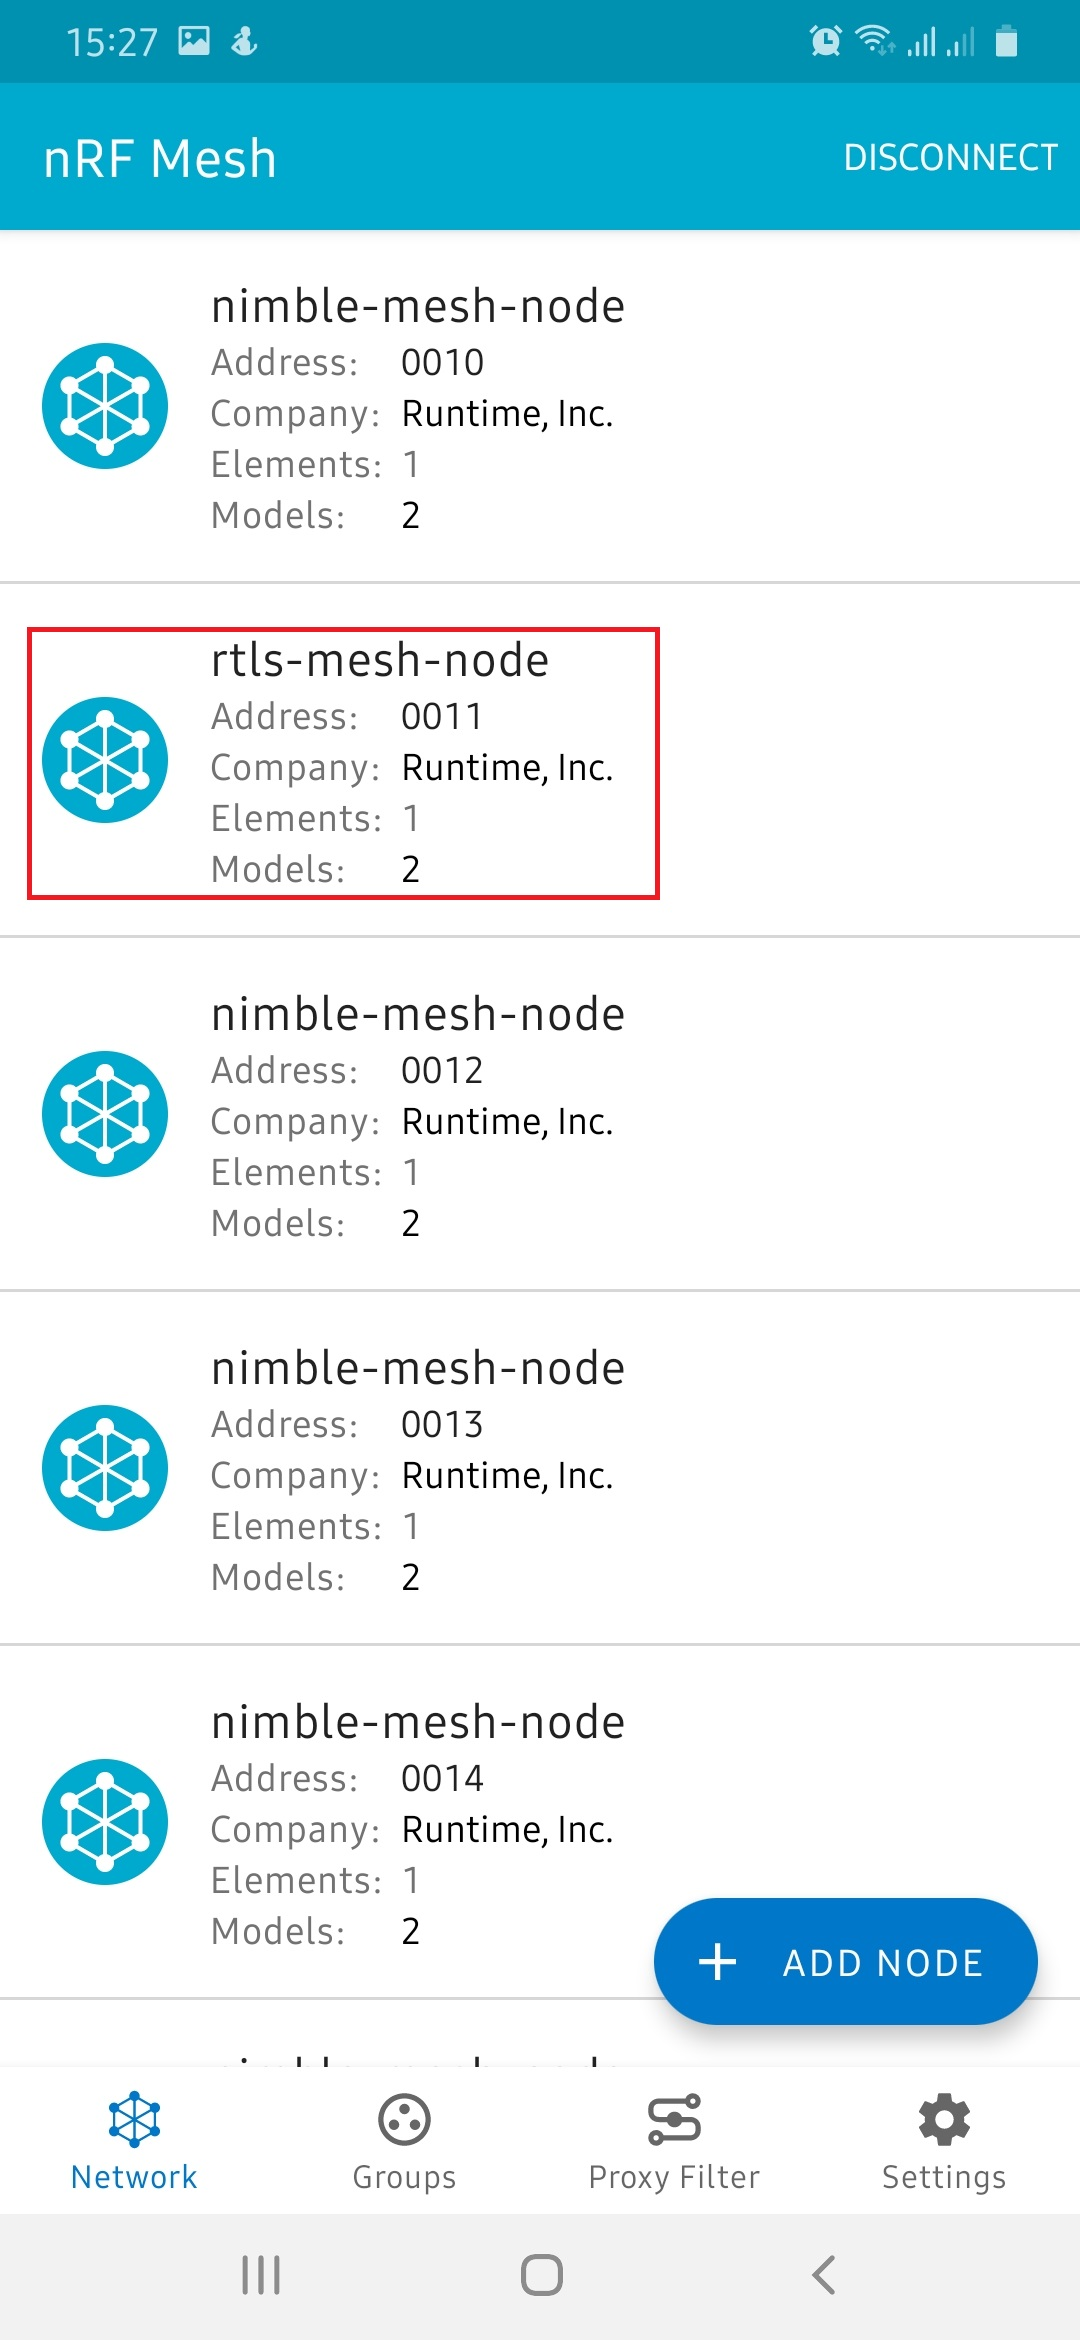
\includegraphics[width=0.9\linewidth]{nRF_Mesh_04.jpg}
            \caption{Bluetooth mesh node list}
            \label{fig:bluetooth_mesh_node_list}
        \end{subfigure}
        \begin{subfigure}[b]{0.24\linewidth}
            \centering
            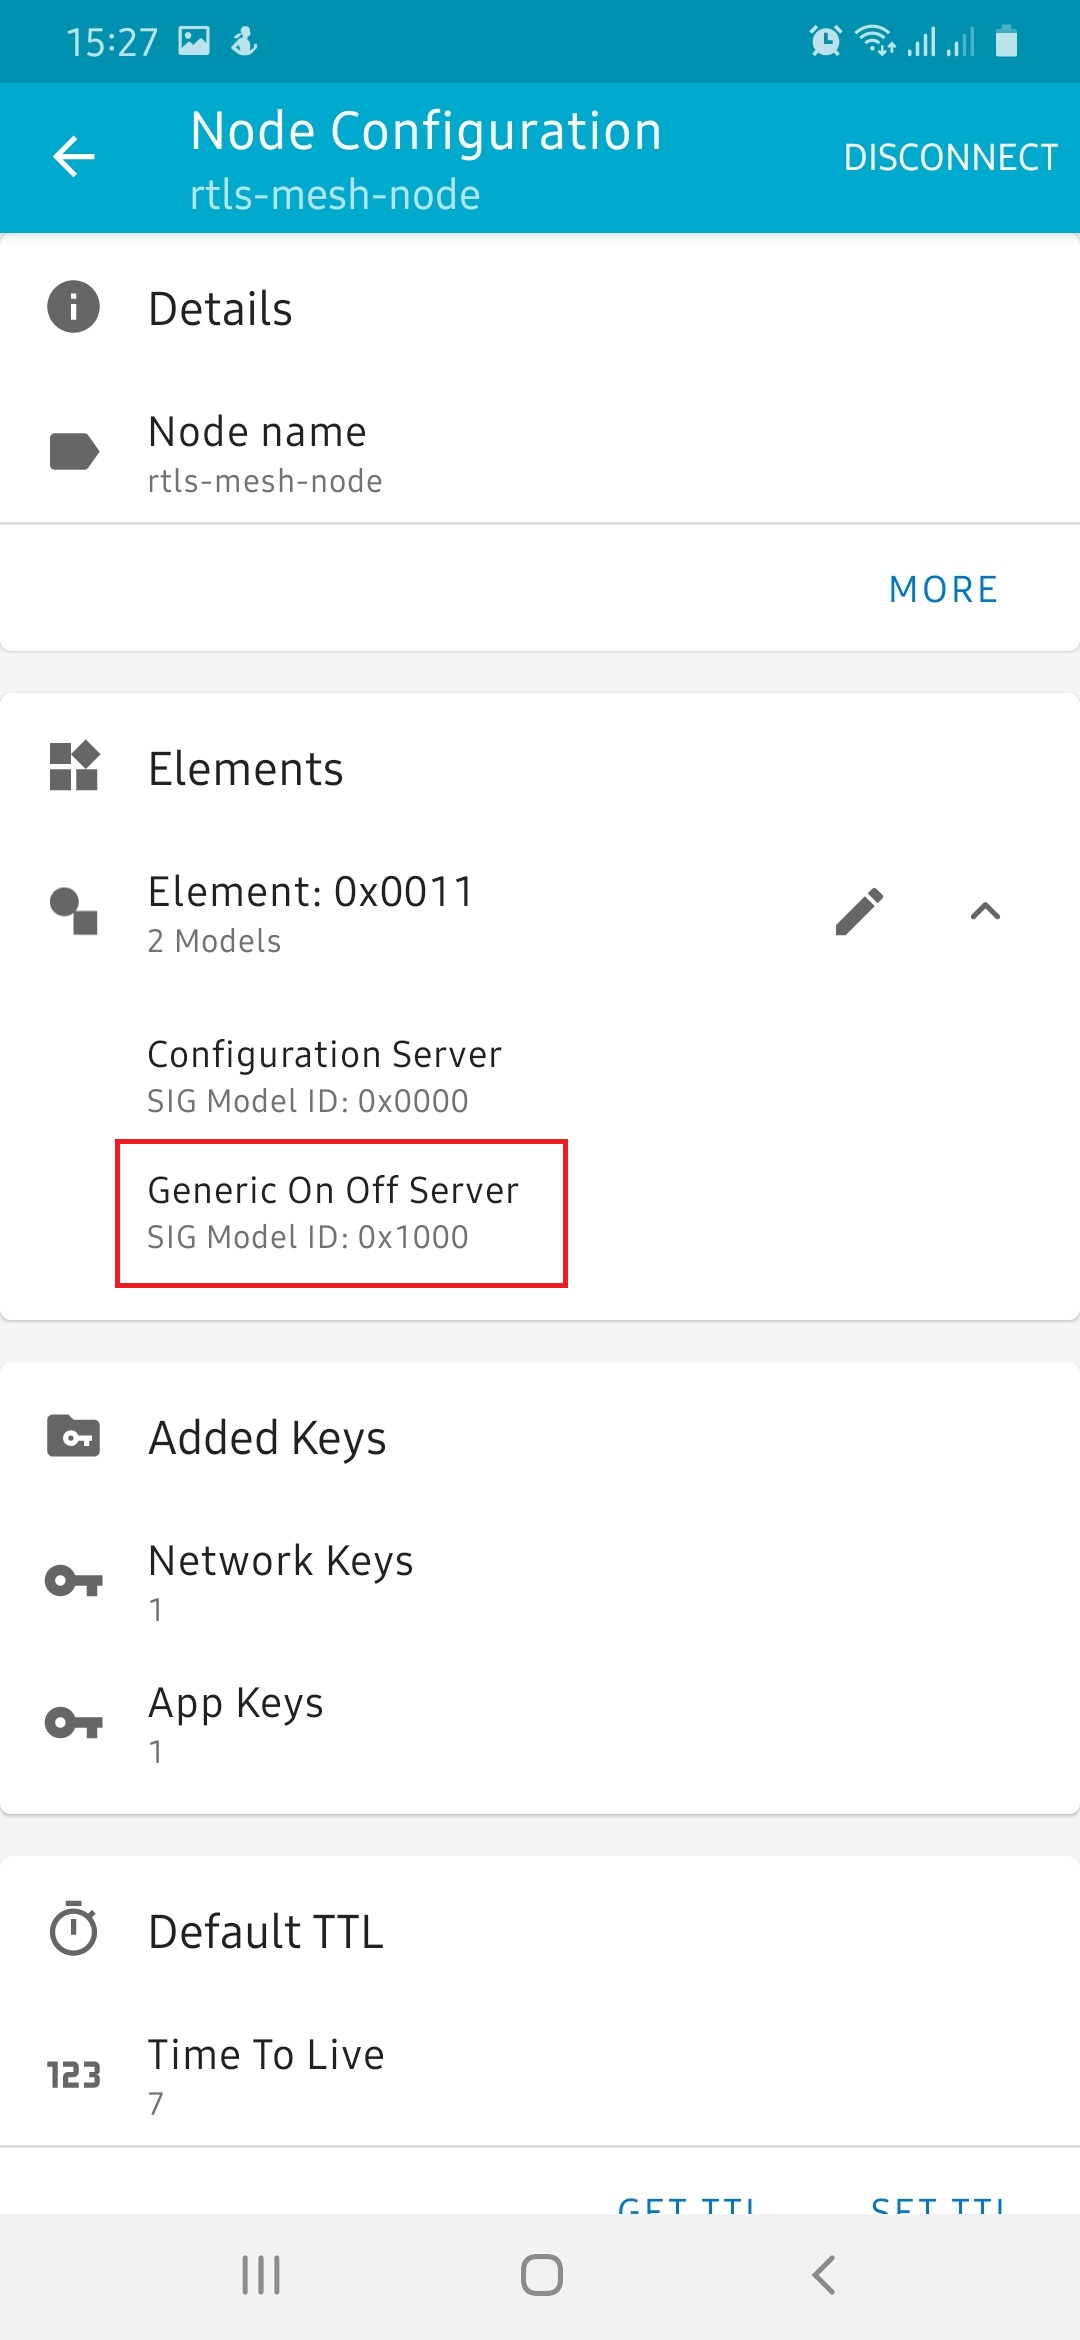
\includegraphics[width=0.9\linewidth]{nRF_Mesh_05.jpg}
            \caption{Node information tab}
            \label{fig:node_element}
        \end{subfigure}
        \begin{subfigure}[b]{0.24\linewidth}
            \centering
            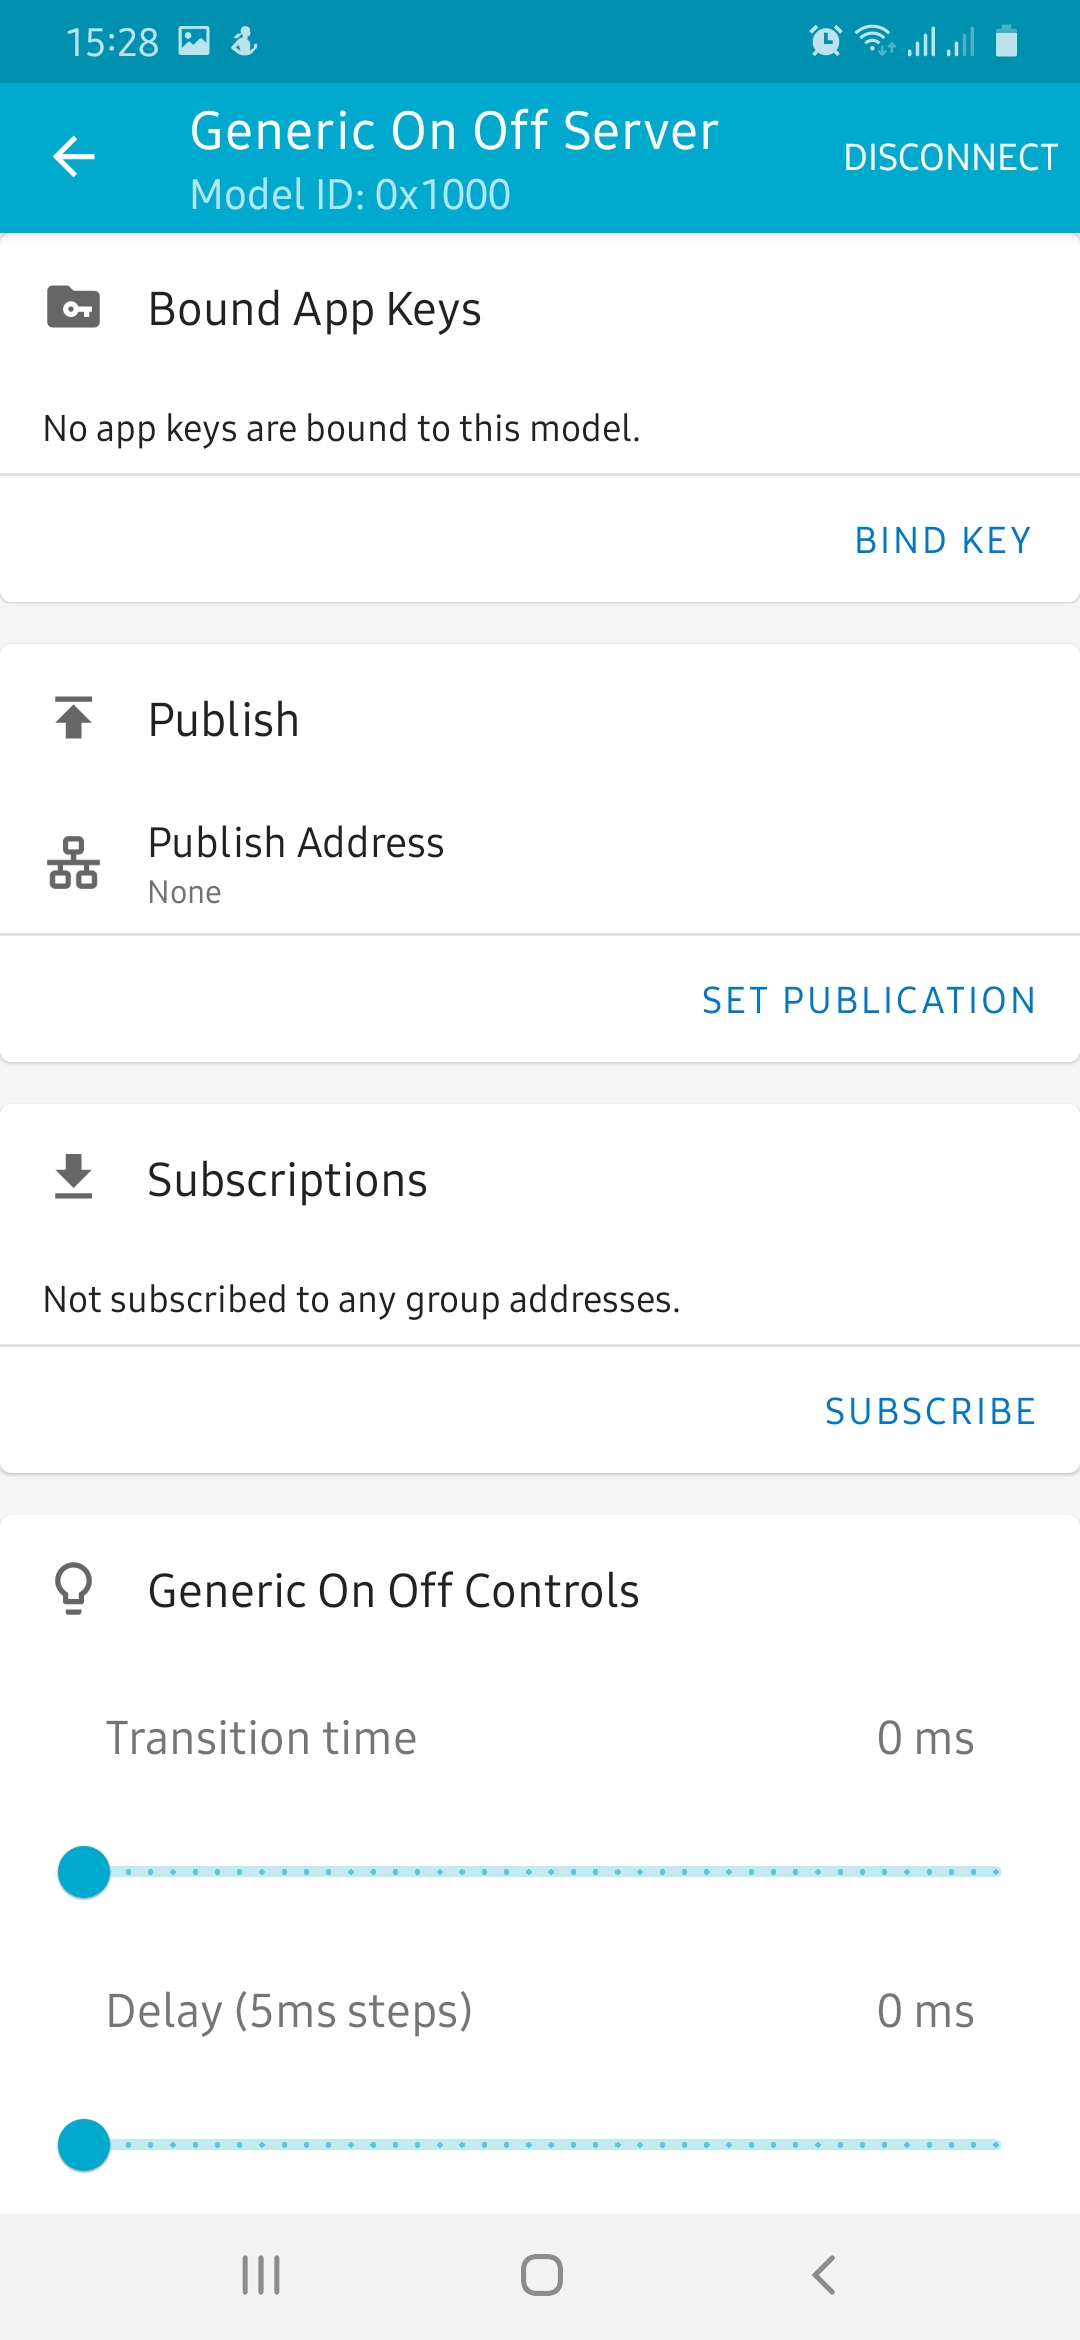
\includegraphics[width=0.9\linewidth]{nRF_Mesh_06.jpg}
            \caption{Element before configuration}
        \end{subfigure}
        \begin{subfigure}[b]{0.24\linewidth}
            \centering
            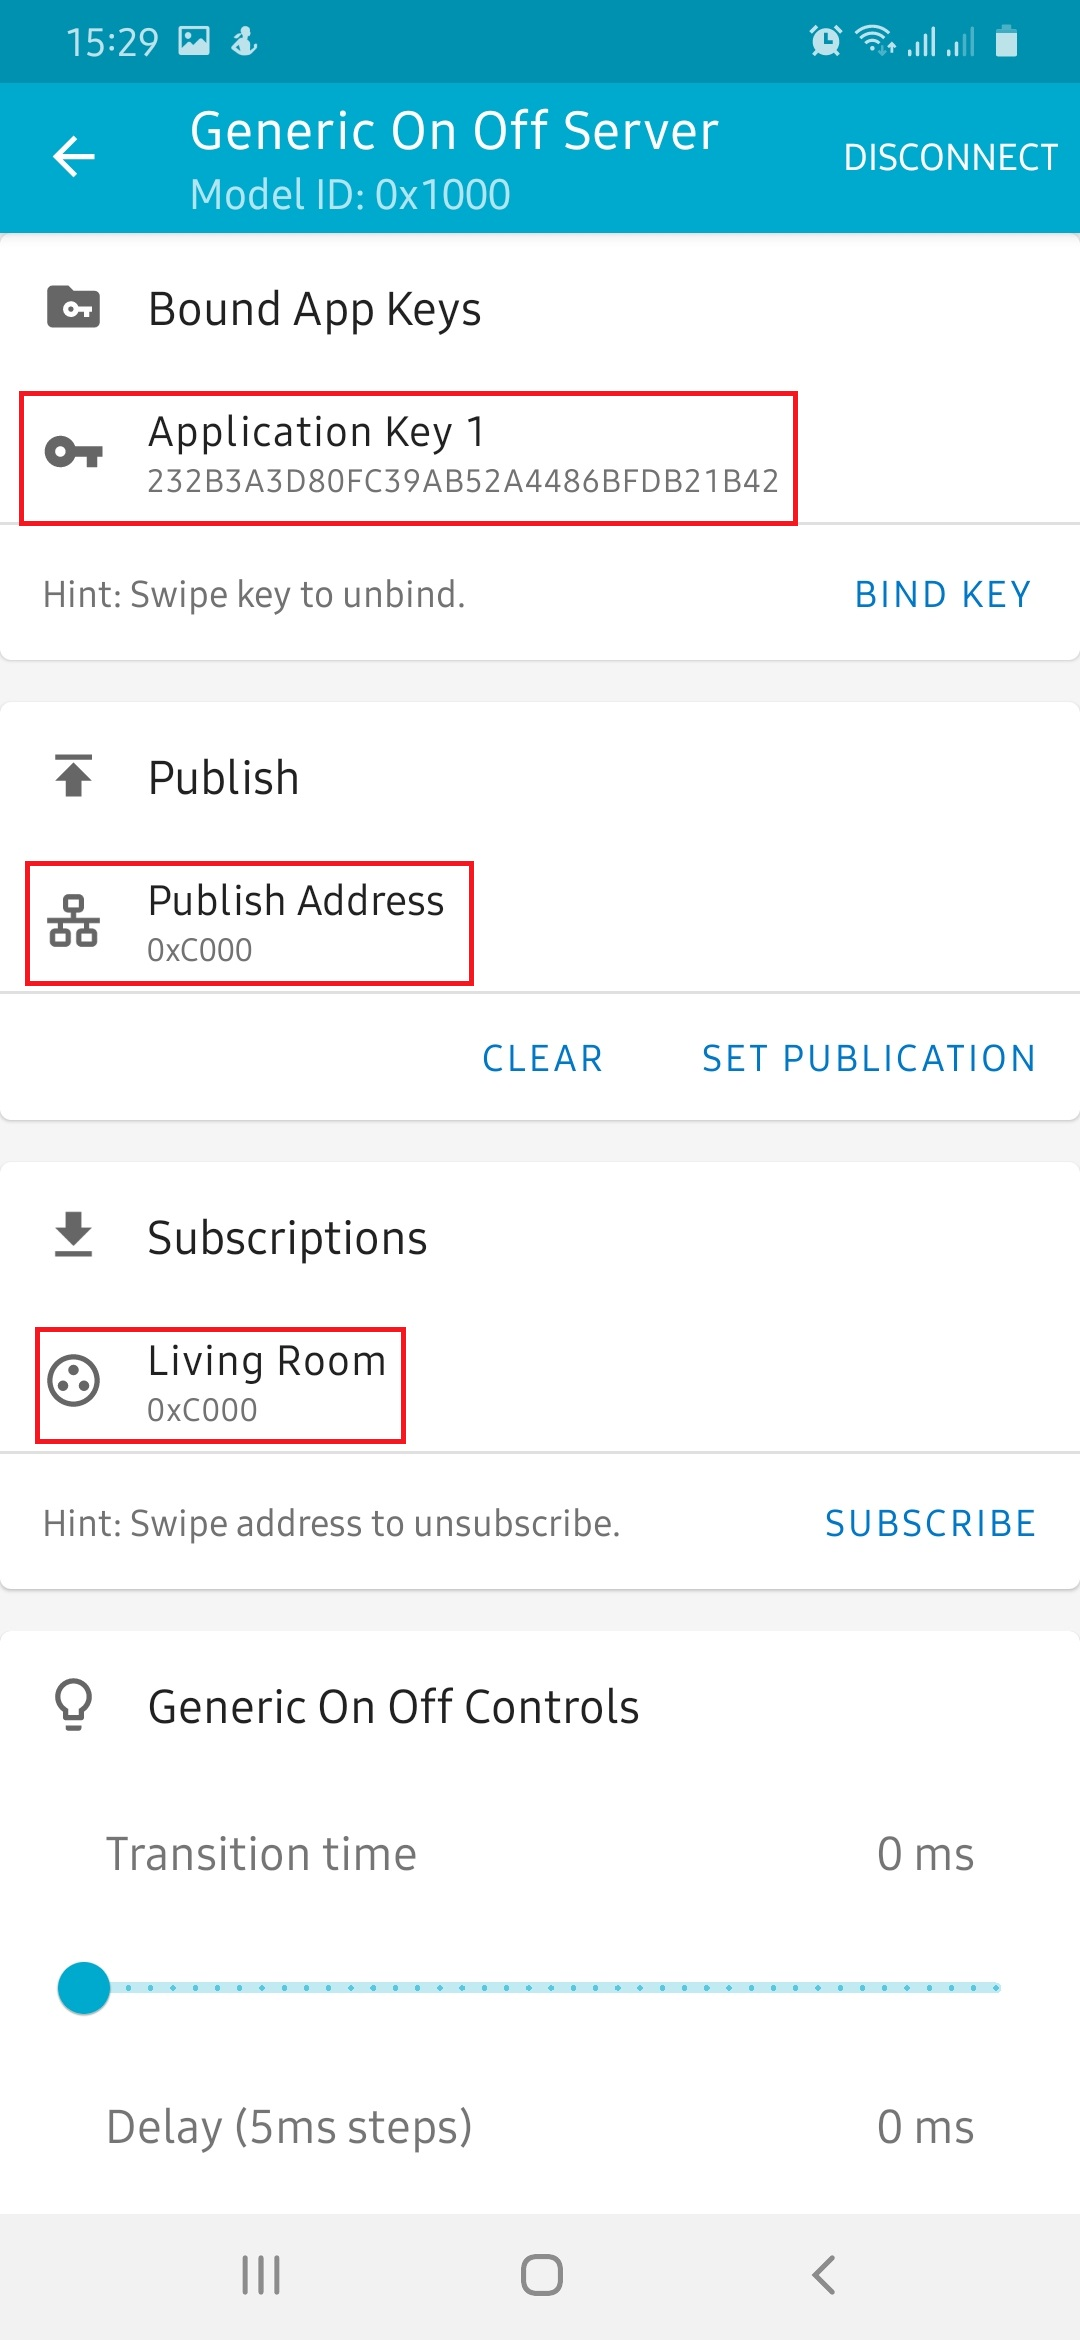
\includegraphics[width=0.9\linewidth]{nRF_Mesh_07.jpg}
            \caption{Element after configuration}
        \end{subfigure}
    \end{figure}
\end{frame}

\section{Hardware}
\begin{frame}
    \myframetitle{Hardware: Battery Charger Circuit + Buck Converter}
    \begin{figure}[H]
        \centering
        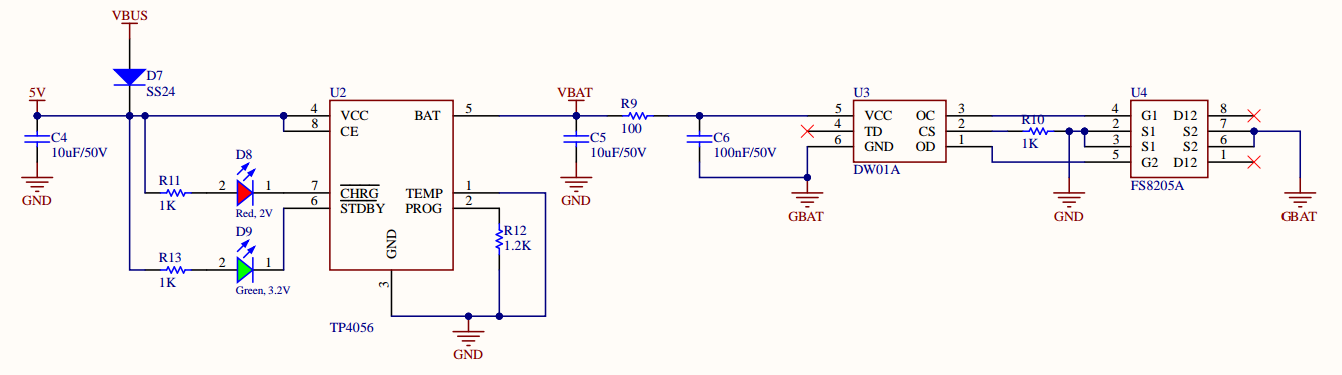
\includegraphics[width=0.8\textwidth]{battery_charger_circuit.png}
        \caption{Battery charger circuit}
    \end{figure}
    \begin{figure}[H]
        \begin{center}
            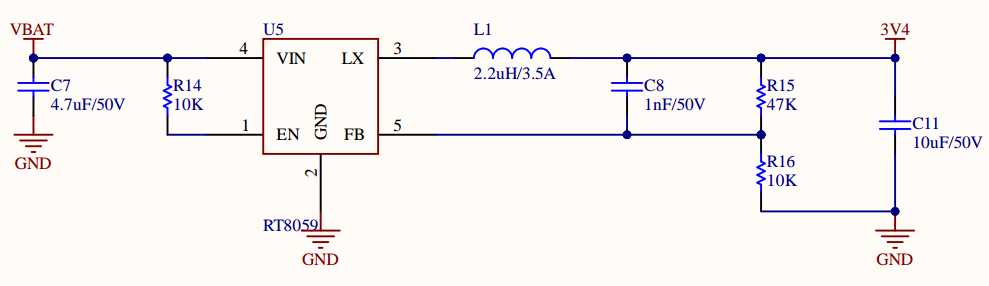
\includegraphics[width=0.8\textwidth]{voltage_set_down_converter.png}
        \end{center}
        \caption{Voltage step-down circuit}
        \label{fig:voltage_set_down_converter}
    \end{figure}
\end{frame}

\begin{frame}
    \myframetitle{Hardware: RTLS Board}
    \begin{figure}[H]
        \centering
        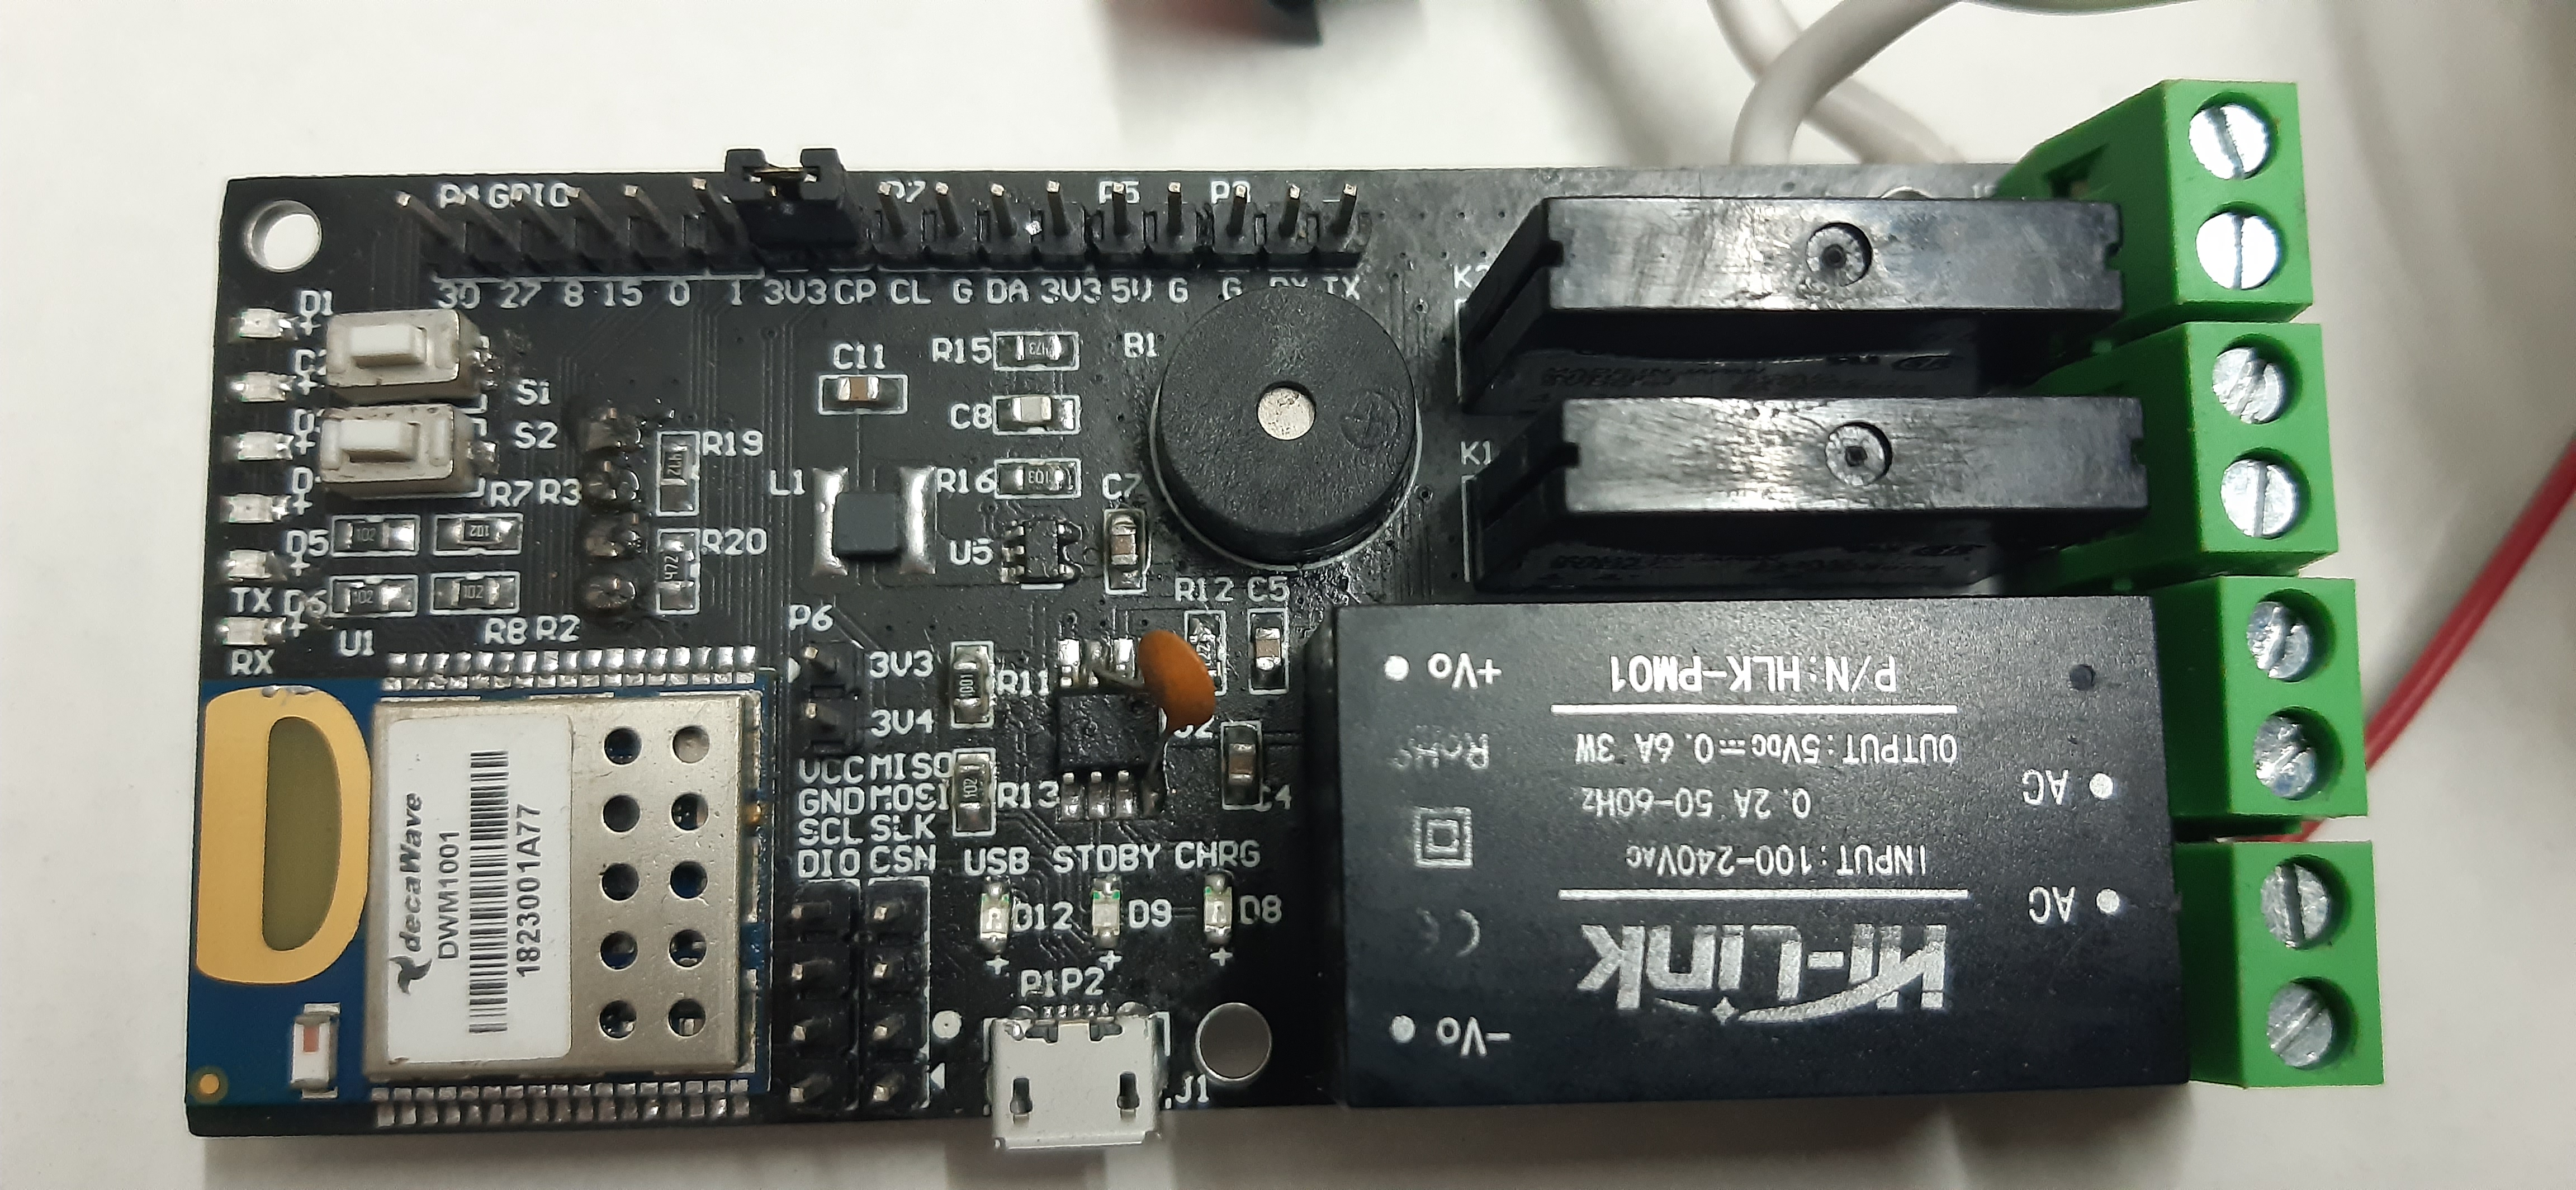
\includegraphics[width=0.5\textwidth]{rtls_anchor_hw_upper.jpg}
        \caption{RTLS anchor board upper face}
    \end{figure}
    \begin{figure}[H]
        \centering
        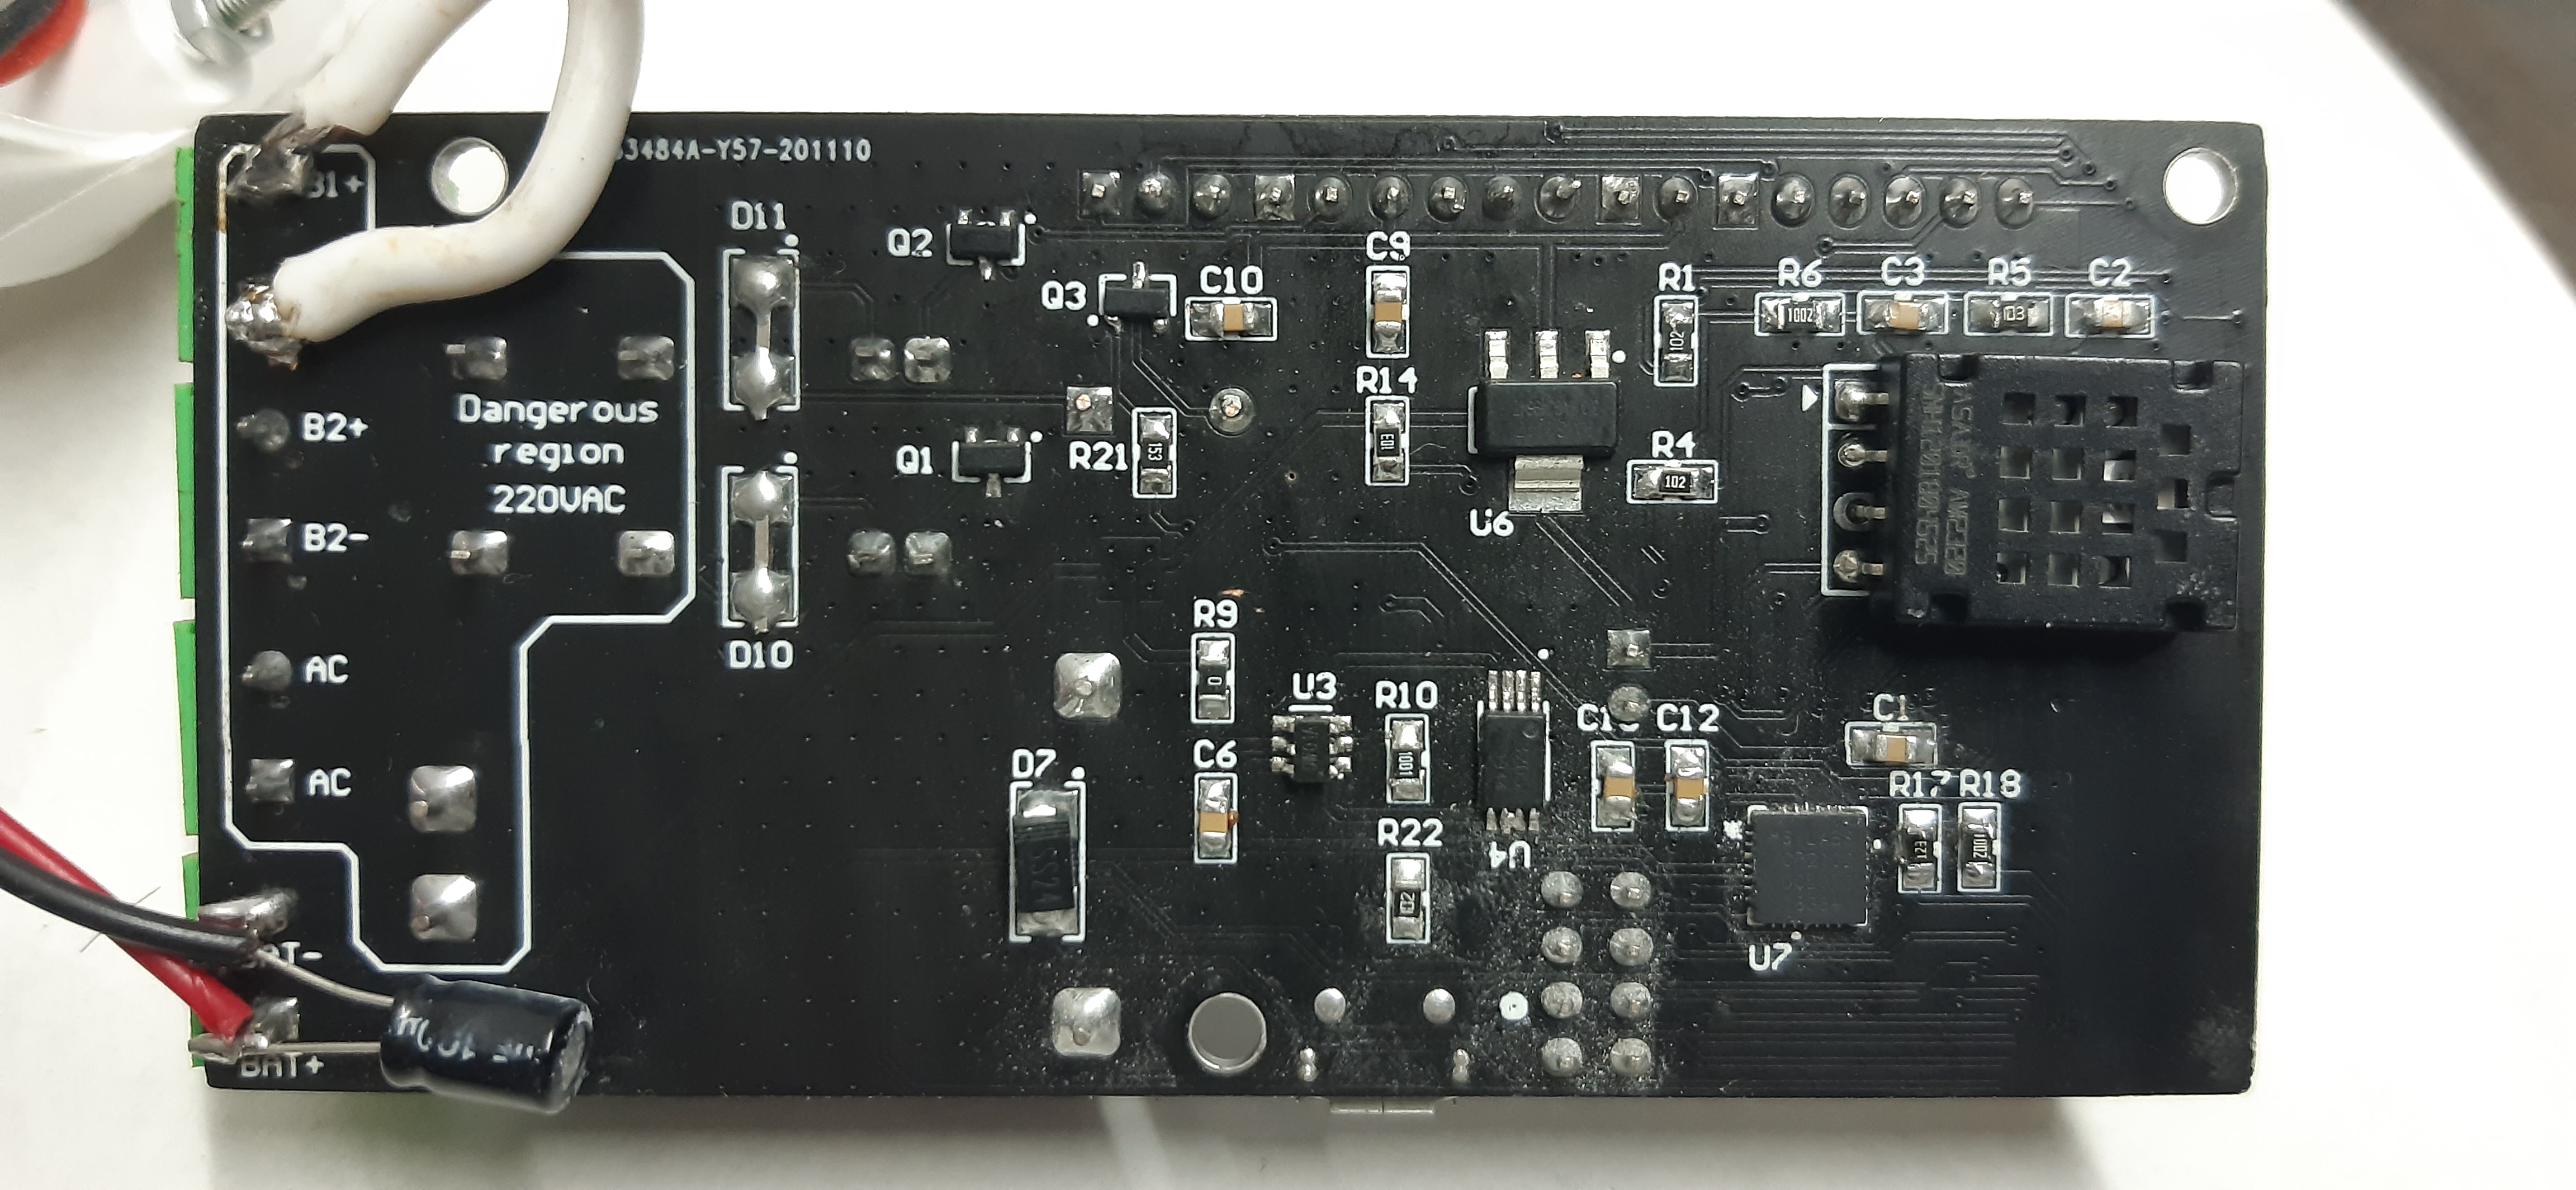
\includegraphics[width=0.5\textwidth]{rtls_anchor_hw_lower.jpg}
        \caption{RTLS anchor board lower face}
    \end{figure}
\end{frame}

\section{Software}

\begin{frame}
    \myframetitle{Software: Gateway}
    \begin{figure}[H]
        \centering
        \begin{subfigure}[b]{0.3\linewidth}
            \centering
            \includegraphics[width=1\textwidth]{MAVLink_over_UART.png}
            \caption{MAVLink/UART stack}
        \end{subfigure}
        \begin{subfigure}[b]{0.6\linewidth}
            \centering
            \includegraphics[width=0.7\textwidth]{gateway_software.png}
            \caption{Gateway software component}
        \end{subfigure}
    \end{figure}
    \begin{figure}[H]
        \centering
        \includegraphics[width=0.9\textwidth]{gateway_firmware.png}
        \caption{Gateway firmware component}
    \end{figure}
\end{frame}

\begin{frame}
    \myframetitle{Software: MQTT}
    \begin{figure}[H]
        \centering
        \includegraphics[width=0.7\textwidth]{mqtt-publish-subscribe.png}
        \caption{MQTT publish-subscribe}
    \end{figure}
    \begin{figure}[H]
        \centering
        \includegraphics[width=0.9\textwidth]{mqtt_json_string.png}
        \caption{MQTT messages}
    \end{figure}
\end{frame}

\begin{frame}
    \myframetitle{Software: System Control and Management}
    \begin{figure}[H]
        \centering
        \includegraphics[width=1\textwidth]{system_control_and_manage_application.png}
        \caption{System Control and Management}
    \end{figure}
\end{frame}

\begin{frame}
    \myframetitle{Software: System Control and Management}
    \begin{figure}[H]
        \centering
        \includegraphics[width=0.5\textwidth]{control_and_manage_pannel.png}
        \caption{Node tab}
    \end{figure}
\end{frame}

\section{System evaluation}

\begin{frame}
    \myframetitle{SE: System Overview}
    \begin{figure}[H]
        \centering
        \includegraphics[width=0.6\textwidth]{system_overview.png}
        \caption{Whole system overview}
        \label{fig:system_overview}
    \end{figure}
\end{frame}

\begin{frame}
    \myframetitle{SE: Static Tag in Single-cell Environment}
    \begin{figure}[H]
        \centering
        \includegraphics[width=0.75\textwidth]{system_overview_phy.png}
        \caption{Scenario 1}
        \label{fig:scenario_1}
    \end{figure}
\end{frame}

\begin{frame}
    \myframetitle{SE: Static Tag in Single-cell Environment}
    \begin{figure}[H]      
        \centering
        \includegraphics[width=1\textwidth]{arena_00.jpg}
        \caption{Experimental arena}
        \label{fig:arena_00}
    \end{figure}
\end{frame}

\begin{frame}
    \myframetitle{SE: Static Tag in Single-cell Environment}

    \begin{columns}
    \column{0.5\textwidth}
    \begin{table}[ht]
        \centering
        \begin{tabular}{|c|>{\centering\arraybackslash}p{0.5cm}|>{\centering\arraybackslash}p{0.5cm}|>{\centering\arraybackslash}p{0.5cm}|}
        \hline
        \backslashbox{y}{x}  &  3 & 7 & 10 \\ \hline
        0 &  0.2 &  0.28 &  0.25  \\ \hline
        2 &  0.14 &  0.13 &  0.18  \\ \hline
        4 &  0.22 &  0.19 &  0.27  \\ \hline
        \end{tabular}
        \caption{Vendor system error}
        \label{table:vendor_rms_error}
    \end{table}
    \column{0.5\textwidth}
    \begin{figure}[H]     
        \centering
        \includegraphics[width=1\textwidth]{rms_error.png}
    \end{figure}
    \end{columns}
    \begin{columns}
        \column{0.5\textwidth}
        \begin{table}[H]
            \centering
            \begin{tabular}{|c|>{\centering\arraybackslash}p{0.4cm}|>{\centering\arraybackslash}p{0.5cm}|>{\centering\arraybackslash}p{0.5cm}|>{\centering\arraybackslash}p{0.5cm}|}
            \hline
            \backslashbox{y}{x}  &  1.2 & 4.8 & 9.6 & 10.8 \\ \hline
            0.6 &  0.10 & 0.20&  0.13 &  0.12  \\ \hline
            1.2 &  0.13 & 0.18&  0.17 &  0.16  \\ \hline
            2.4 &  0.09 & 0.10&  0.11 &  0.22  \\ \hline
            \end{tabular}
            \caption{Proposed system error}
            \label{table:proposed_rms_error}
        \end{table}
        \column{0.5\textwidth}
        \begin{figure}[H]     
            \centering
            \includegraphics[width=1\textwidth]{result_static.png}
        \end{figure}
    \end{columns}
\end{frame}

\begin{frame}
    \myframetitle{SE: Mobile Tag in Single-cell Environment}
    \begin{figure}[H]
        \centering
        \includegraphics[width=1\textwidth]{result_square.png}
        \caption{Rectangle movement result}
        \label{fig:result_rectangle}
    \end{figure}
\end{frame}

\begin{frame}
    \myframetitle{SE: Mobile Tag in Multi-cell Environment}
    \begin{figure}[H]
        \centering
        \includegraphics[width=1\textwidth]{system_overview_phy_full.png}
        \caption{Scenario 3}
        \label{fig:scenario_3}
    \end{figure}
\end{frame}

\begin{frame}
    \myframetitle{SE: Mobile Tag in Multi-cell Environment}
    \begin{figure}[H]      
        \centering
        \includegraphics[width=1\textwidth]{arena_03.jpg}
        \caption{Experimental arena}
        \label{fig:node_4_5_6_7}
    \end{figure}
\end{frame}

\begin{frame}
    \myframetitle{SE: Mobile Tag in Multi-cell Environment}
    \begin{figure}[H]
        \centering
        \includegraphics[width=1\textwidth]{path.png}
        \caption{Multi-cell movement result}
        \label{fig:multi_cell_movement_result}
    \end{figure}
\end{frame}

\begin{frame}
    \myframetitle{SE: IoT Service}
    \begin{figure}[H]
        \centering
        \includegraphics[width=0.9\textwidth]{result_remote_control_off_gui.png}
    \end{figure}
    
    \begin{figure}[H]
        \centering
        \includegraphics[width=0.9\textwidth]{result_remote_control_on_gui.png}
    \end{figure}
\end{frame}

\begin{frame}
    \myframetitle{SE: IoT Service}
    \begin{figure}[H]
        \centering
        \includegraphics[width=0.5\linewidth]{result_remote_control_off_result.jpg}
    \end{figure}
    \begin{figure}[H]
        \centering
        \includegraphics[width=0.5\linewidth]{result_remote_control_on_result.jpg}
    \end{figure}
\end{frame}

\section{Summary}
\begin{frame}
    \myframetitle{Summary}
    Achievement:
    \begin{itemize}
        \item Design and implement an indoor localization system using UWB. \\The performance => similar in comparison with the vendor system.
        \item Build a system to manage and control the localization system based on a Bluetooth mesh network.
        \item The mesh network also provides remote control service.
    \end{itemize}
    Further Development:
    \begin{itemize}
        \item Improve the system stability.
        \item Test and deploy the network with more nodes.
        \item Test and deploy the network with more cells.
        \item Optimize system to extend battery life.
        \item Design and implement a reliable protocol based on best-effort broadcast service provided by Bluetooth mesh network.
        \item Try different distance measurement methods.
        \item Try different position estimation methods.
    \end{itemize}
\end{frame}

\end{document}